\documentclass[journal,onecolumn]{IEEEtran}
\renewcommand{\baselinestretch}{1.45}
\setlength{\parindent}{13pt}


\usepackage{mathrsfs}
\usepackage{booktabs}
\usepackage{cite}
\usepackage[justification=centering]{caption} % Center the caption
\usepackage{amssymb}
\usepackage{amsmath}
\usepackage{graphics}
\usepackage{color}
\usepackage{epsfig}
\usepackage{graphicx}
\usepackage{amsthm}
\usepackage{float}
\usepackage{subfigure}
\usepackage{amsmath}
\usepackage{amsfonts}
\usepackage{placeins}
\usepackage{lettrine} % Package for dropped capital letters


\allowdisplaybreaks[4]

\title{\LARGE Data-Driven Model-Free Adaptive Sliding Mode Control for Multi DC Motor Speed Regulation}

\author{bim}

\begin{document}
\maketitle

\begin{abstract}
    This paper proposes the distributed data-driven model-free adaptive sliding mode control approach to address the consensus problem of nonlinear multi-agent systems. Firstly, the equivalent data model for each agent is constructed using the compact-form dynamic linearization (CFDL) technique. Secondly, by utilizing process information from neighboring agents, the novel sliding surface is employed to ensure the boundedness of distributed measurement error based on stability analysis. Subsequently, a distributed model-free adaptive sliding mode controller is developed for accurate consensus tracking. Finally, the effectiveness of the proposed control approach is verified through experiments on multi DC motor system.
\end{abstract}

% It would be more appropriate to rephrase it using a relative clause introduced by 
% “which.” This would avoid making the sentence appear too lengthy.

\section*{Keywords}
Data-driven control, model-free adaptive sliding mode control, nonlinear multi-agent systems, multi DC motor speed control.

\section{Introduction}\label{section:1}

Due to the excellent capabilities and coordination efficiency of distributed multi-agent systems (MASs) in various applications such as sensor network, transportation systems, agriculture monitoring and industrial process systems \cite{1,2,3}, MASs have attracted significant attention. Over the past few years, one of the main challenges for collaborative control \cite{4,5,6} is to handle consensus problem. It means that all agents can follow the same trajectory from different initial values. However, traditional model-based control strategies are not suitable for complex systems that are difficult to model accurately. Despite their effectiveness in certain scenarios, traditional control strategies \cite{10,11,12,13} heavily depend on precise system models and the modeling process becomes increasingly challenging as technology grows rapidly. Under such circumstances, it becomes difficult to solve practical problems using the above schemes. In modern industrial environments, vast amounts of process information often containing implicit and complex dynamic behaviors of the system are continuously generated and stored during operation. As a result, there has been a growing interest in alternative control methods that rely on data modeling. 

Therefore, how to use this data to achieve system consensus control has become a powerful new topic. The data-driven control \cite{17,18,19,20} refers to control systems utilizing system I/O data solely. Various data-based approaches have been developed, including model-free adaptive control, iterative learing control, virtual reference feedback tuning \cite{21}, PID control \cite{22} and others. Among these,  the model-free adaptive control approach \cite{23,24,25} has been proposed, and has a great significance in addressing the aforementioned challenges. The design process relies solely on I/O data of the system, significantly avoiding the reliance on mathematical models. The algorithm has proven effective in practical domains such as motor systems, chemical industries, and machinery, demonstrating the adaptability and usefulness of the algorithm. 

Alternatively, sliding mode control \cite{26} has emerged as a highly attractive approach for the control researchers due to its robustness to parameter uncertainties and its capability to ensure fast responses. Currently, the novel sliding mode control method based on I/O data is presented in \cite{27}, which eliminate the need for explicit system models. 
Although considerable progress has been made in controlling nonlinear MASs, the dynamic couplings and complex nonlinear behaviors among agents \cite{14} can be challenging practical implementation.

However, the effectiveness of existing approaches \cite{31,32,33,34} is limited in highly uncertain environments because they typically rely on input-affine structures with known or partially known dynamics.
How to achieve consensus tracking problem utilizing the model-free adaptive sliding mode controller approach for nonlinear MASs remains an open question.

Inspired by the above discussions, this paper proposes a data-driven model-free adaptive sliding mode control scheme. The contributions of this paper are structured as follows:

\begin{enumerate}

    \item This paper establishes the model-free adaptive sliding mode control approach, which enables consensus tracking in nonlinear MASs, even under system uncertainties and unknown dynamics.
    
    \item The method utilizes CFDL to construct equivalent data models based purely on input-output data. This allows for the systematic design of controllers for each agent without requiring internal system knowledge, making it highly practical for real-time applications.
    
    \item A novel distributed sliding surface is developed using neighboring agent process data. This structure ensures the boundedness of measurement errors and enhances the robustness and convergence of the system through a designed stability mechanism.

\end{enumerate}


    The following sections will outline the remaining content of this paper:
    section II provides preliminaries and problem formulation, Section III presents The main results, Section IV shows simulation results and performance analysis, demonstrating the effectiveness of the proposed method under distinct operating conditions. At the end, conclusions are summarized in Section V.
% -----------------------------------------------------------------------------


\section{Preliminaries and problem formulation}\label{section:2}
\subsection{Directed Graph Theory}

\indent The directed graph $ \mathcal{G} = (\mathcal{V}, \mathcal{E}, \mathcal{A}) $ is employed to describe the information exchange between agents. Here, $ \mathcal{A} = [a_{ij}] \in \mathbb{R}^{N \times N} $ represents the adjacency matrix, $ \mathcal{V}=\{v_1, v_2,\dots,v_N\} $ is the set of vertices, and $ \mathcal{E} = [(v_j,v_i)|v_i \in \mathcal{V} ] \subseteq \mathcal{V} \times \mathcal{V}$ is the set of edges. Moreover, $ \mathcal{N}(i) = \{j \in \mathcal{V} |(i,j) \in \mathcal{E}\} $ denotes the neighbor set of agent $ i $, where $ a_{i j} \neq 0$. No self-loop is allowed in this article, which means $(i, i) \notin \mathcal{E}$ for any $ i \in \mathcal{V} $, $ a_{ii}=0$. Furthermore, the degree matrix $ K = diag(k_1,\dots,k_N)$. If $ k_i > 0$, agent $ i $ can directly obtain the information from the leader. The Laplacian matrix $ L $ is defined as $ L = (\mathcal{D}-\mathcal{A})$, here $\mathcal{D} = diag({d_1,\dots,d_N})$ and $d_i=\sum_{j=1}^{N} a_{i j}$ denotes the in-degree matrix. Moreover, the graph is strongly connected if the path exists between every pair of vertices.

\subsection{Problem Formulation}

Consider the nonlinear multi-agent systems composed of $ N $ agents:
\begin{equation}
    \label{model 1}
    y_i(k+1) = f_i(y_i(k), u_i(k)), \quad i = 1, 2, \dots, N
\end{equation}
% \noindent 
where $u_i(k) \in \mathbb{R}$ and $y_i(k) \in \mathbb{R}$ represent the system input and output signals of agent $ i $, respectively. $f_i(\cdot)$ signifies an unknown nonlinear function.

Assumption 1: The partial derivative of \( f_i(\cdot) \) with respect to \( u_i(k) \) is continuous.

Assumption 2: The system (\ref{model 1}) satisfies the generalized Lipschitz condition, meaning that if \( \Delta u_i(k) = u_i(k) - u_i(k - 1) \neq 0 \) then \( | \Delta y_i(k + 1) | \leq b |\Delta u_i(k)| \) holds for any \( k \), where \( \Delta y_i(k + 1) = y_i(k + 1) - y_i(k) \).
 

% Under Assumptions 1 and 2, the unknown agent dynamics (\ref{model 1}) can be transformed into the following dynamic linearization model and then the distributed control law will be designed based on it:

Remark 1: The assumptions above are general. Assumption 1 is a general condition for controller design. Assumption 2 implies that the system input rate constrains the system output rate, which is satisfied in many practical systems.

Assumption 3: The communication graph $ \mathcal{G} $ is strongly connected, ensuring that each follower can directly receive information from at least one leader.

Lemma 1\cite{8}: Consider the nonlinear multi-agent system (\ref{model 1}) satisfying above three assumptions. If $ | \Delta u_i(k) | \neq 0 $ holds, then the system can be transformed into the CFDL data model as follows:
\begin{equation}
    \label{model 2}
    \Delta y_i(k+1)=\phi_i(k)\Delta u_i(k)
\end{equation}
wherein \(\phi_i(k)\) is called pseudo partial derivative (PPD), satisfying \( | \phi_i(k) | \leq b\).
 
The distributed measurement error of \(\xi_i(k)\) for $N$ agents is established as:
\begin{equation}
    \label{model 3}
    \xi_i(k) = \sum_{j \in N_i} a_{ij}( y_j(k)-y_i(k)) + d_i(y_d(k) - y_i(k ))
\end{equation}
if the agent $ i $ can receive data from the leader, then $d_i=1$; otherwise, $d_i=0$. Additionally, $y_d(k)$ represents the reference trajectory. 

Remark 2: The CFDL technique requires no prior knowledge about the system dynamic model. Moreover, the dynamic behavior of time-varying PPD may be highly complex and difficult to verify. 
 

\section{Main Results}




\begin{figure}[H]
    \centering
    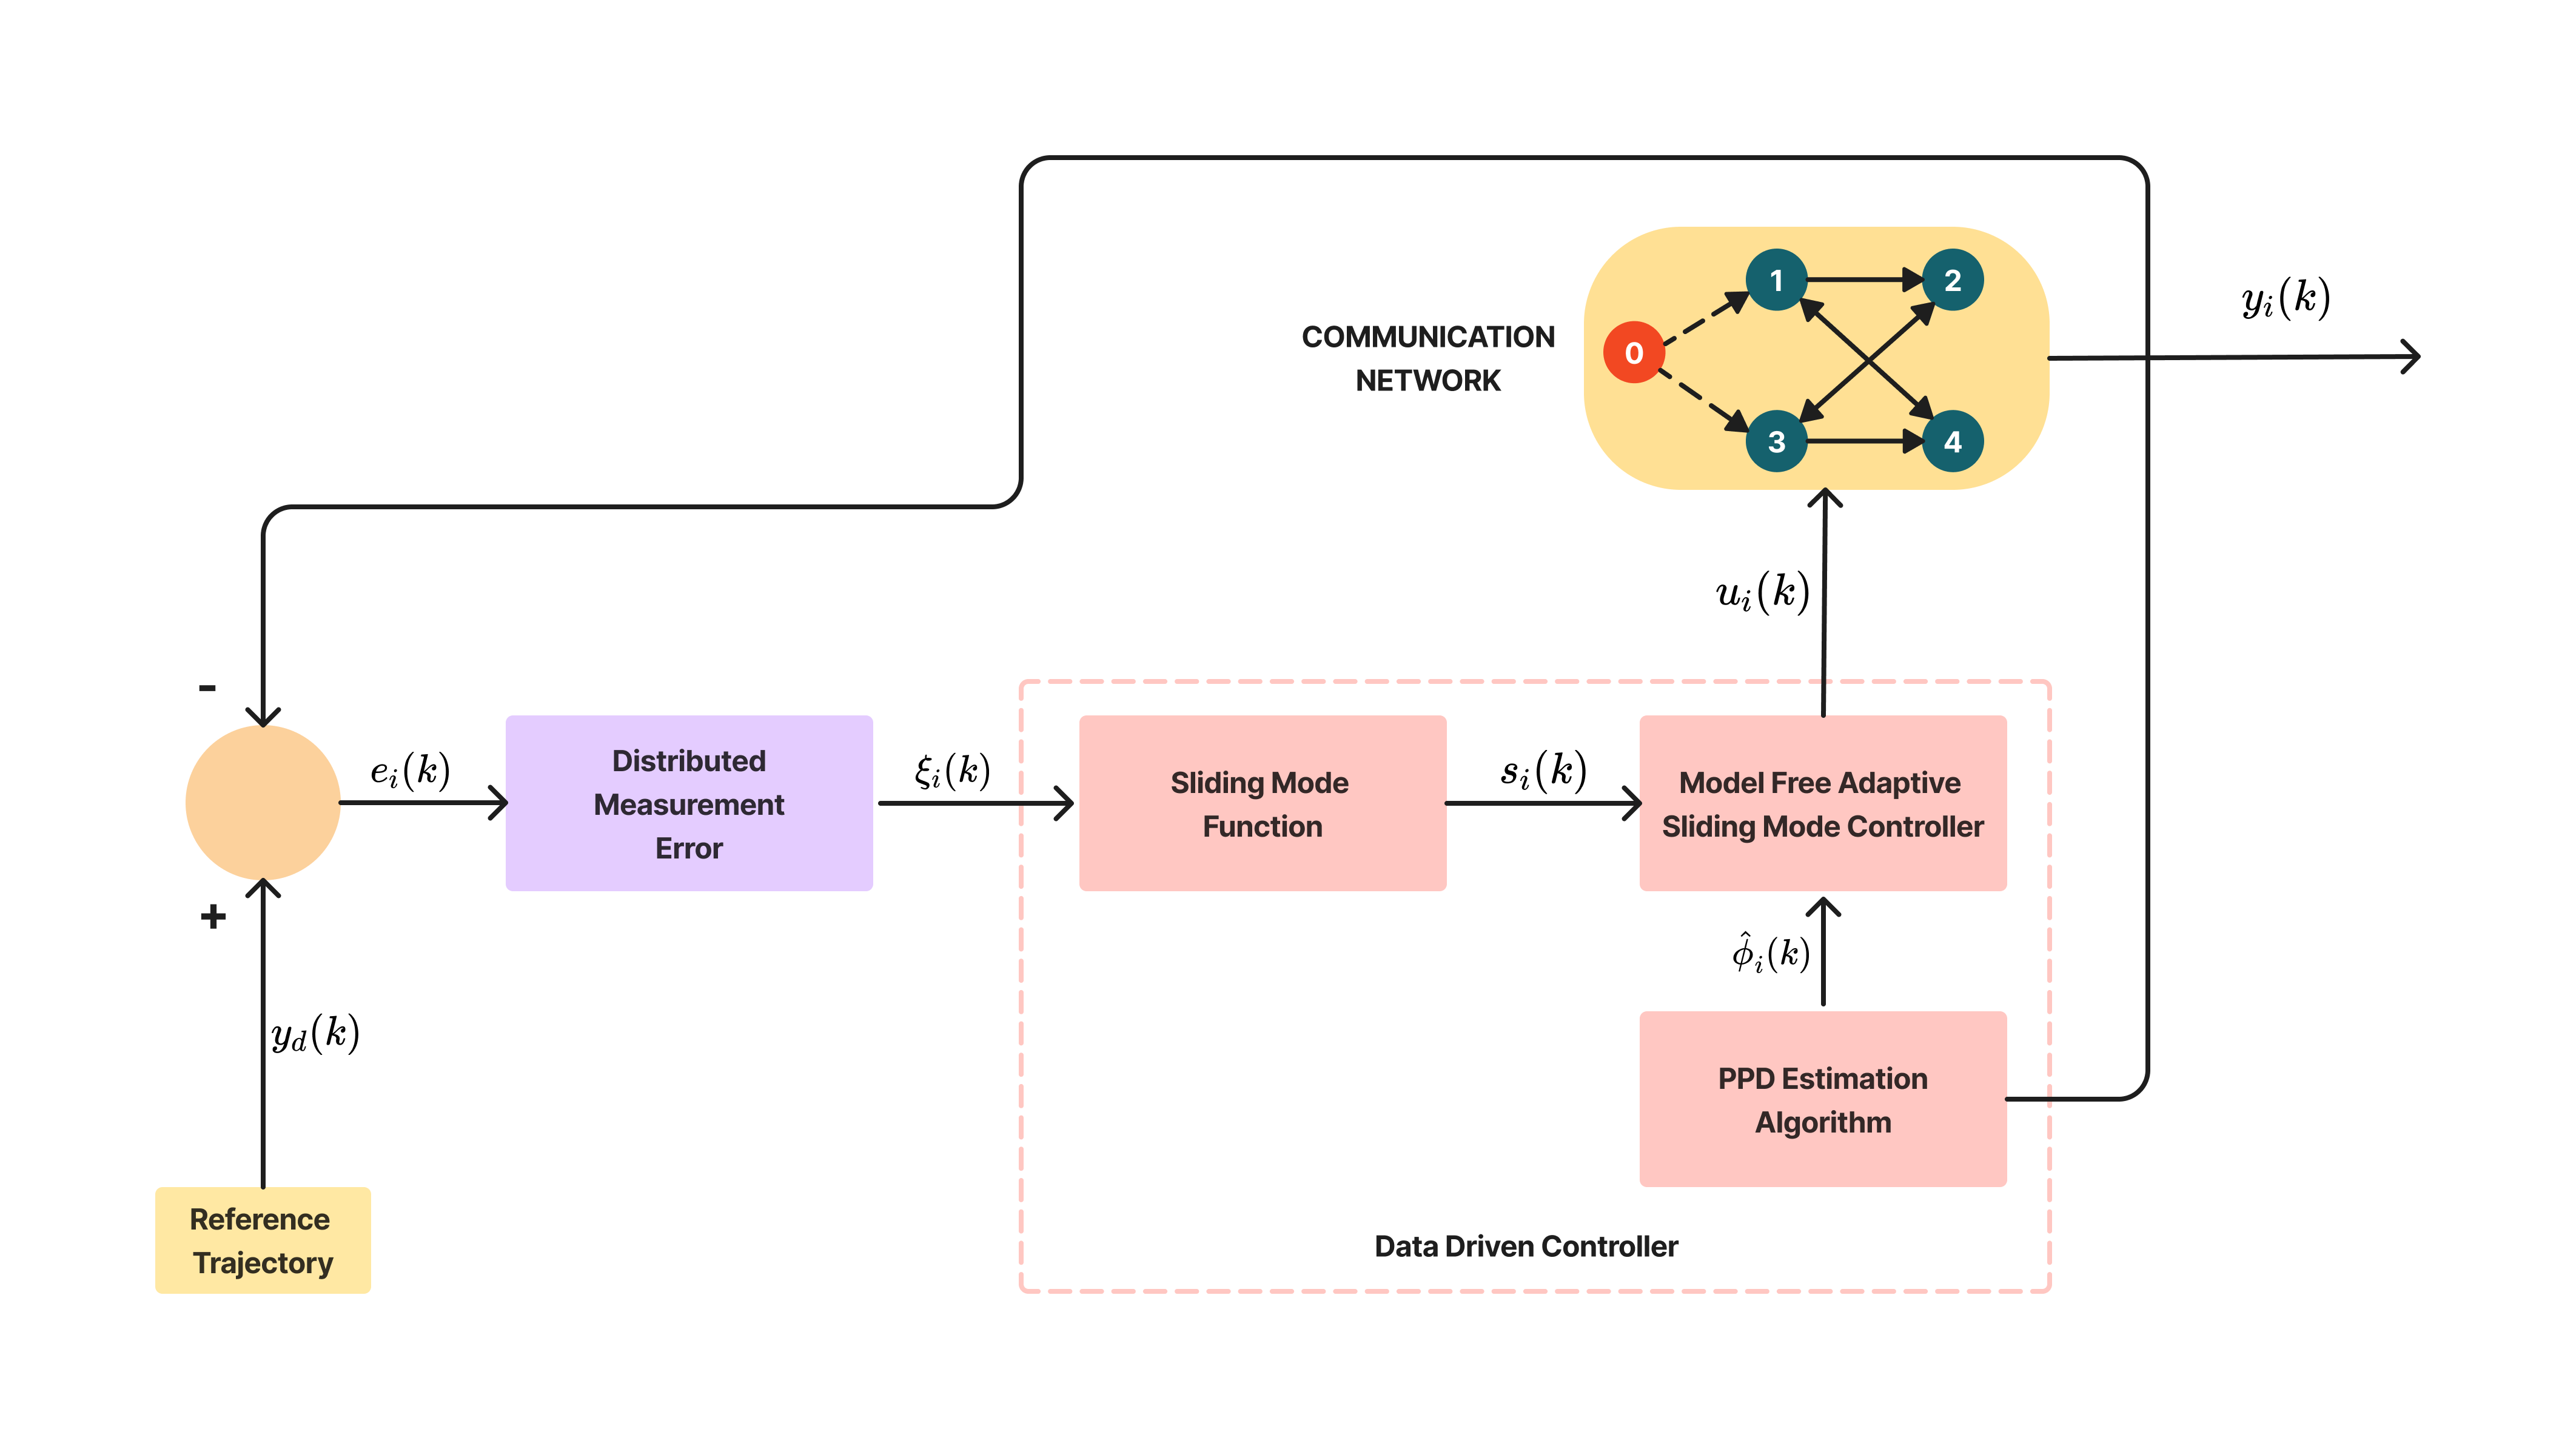
\includegraphics[width=0.8\textwidth]{diagram.png}
    \caption{Block diagram.}
    \label{fig:diagram} % Label for referencing the figure
\end{figure}

This section is devided in two parts. The first part introduces the model-free adaptive controller design, which is based on the CFDL technique. The second part introduces the sliding mode controller design, which is formulated based on the distributed measurement error. The overall block diagram of the proposed control scheme is shown in Fig. \ref{fig:diagram}.

\subsection{Model-Free Adaptive Controller Design}


Consider the following PPD criterion function, for the above consensus tracking objective \(\phi_i(k)\):
\begin{equation}
    \label{model 4}
    J(\phi_i(k)) = | \Delta y_i(k) - \phi_i(k)  \Delta u_i(k-1)|^2 + \mu |\phi_i(k) - \hat{\phi}_i(k-1)|^2\
\end{equation}

By utilizing the optimal condition $ \frac{\partial J(\phi_i(k))}{\partial \phi_i(k)}=0 $, the updating law with reset algorithm is derived:
\begin{equation}
    \label{model eq:ppd_parameter}
    \hat{\phi}_i(k) = \hat{\phi}_i(k-1) + \frac{\eta \Delta u_i(k-1) }{\mu + \Delta u_i(k-1)^2}(\Delta y_i(k) - \hat{\phi}_i(k-1) \Delta u_i(k-1))
\end{equation}
\begin{equation}
    \label{reset}
    \hat{\phi}_i(k) = \hat{\phi}_i(1),  \text{ if }  |\hat{\phi}_i(k) | \leq \epsilon \ or \ sign(\hat{\phi}_i(k)) \neq  sign(\hat{\phi}_i(1))
\end{equation}
herein, $\eta \in (0,1)$, $\mu > 0$ represents a positive weight factor. Additionally, $\epsilon$ is a small positive number. Finally, $\hat{\phi}_i(k)$ signifies the estimated value of $\phi_i(k)$.

The following distributed MFAC algorithm is presented:
\begin{equation}
    \label{model eq:mfac}
    u_{i,\text{MFA}}(k) = u_{i,\text{MFA}}(k - 1) + \frac{\rho \hat{\phi}_i(k)}{\lambda + \hat{\phi}_i(k)^2} \xi_i(k)
\end{equation}
where \(\rho\) \(\in\) (0,1) is a step-size constant, which is added to make (\ref{model eq:mfac}) general. 

\subsection{Sliding Mode Controller Design}

To design the sliding mode controller for the system, the sliding surface function is given by:
\begin{equation}
    \label{model eq:sms}
    s_i(k) = \alpha \xi_i(k) - \xi_i(k-1)
\end{equation}
herein $ \alpha > 1$ represents a positive constant.

Furthermore, from ($ \ref{model 2}) $ and ($ \ref{model 3} $), the formula ($ \ref{model 3} $) is updated as
\begin{align}
    \label{model eq:xi_next}
    \xi_i(k+1) =\ & \xi_i(k) - (\sum_{j \in N_i} a_{ij} + d_i ) \phi_i(k) \Delta u_i(k) + \sum_{j \in N_i} a_{ij} \Delta y_j(k) + d_i \Delta y_d(k+1)
\end{align}
wherein $\Delta y_j(k+1)$ is replaced with $ \Delta y_j(k) $ because the data at the next moment cannot be obtained.

% Then, ($ \ref{model eq:sms}  $) is given as

% \begin{align}
%     \label{model eq:sms_next}
%     S_i(k+1) =\ & (\alpha-1)\xi_i(k) - \left(\sum_{j \in N_i} a_{ij} + d_i \right) \phi_i(k) \Delta u_i(k) + \alpha \sum_{j \in N_i} a_{ij} \Delta y_j(k) \nonumber \\
%     &  + d_i \Delta y_d(k+1)
% \end{align}


Therefore, considering ($ \ref{model eq:sms}) $, with the assistance of reaching law $ s_i(k+1) = 0 $, the following equivalent control law can be derived.

\begin{equation}
    \label{model eq:equivalent_control}
    \Delta u_{i,\text{SM}}^{eq} = \frac{\omega \hat{\phi}_i(k)}{\sigma + \hat{\phi}_i(k)^2}\bigg(\frac{\xi_i(k)+ \sum_{j \in N_i}a_{ij} \Delta y_j(k) + d_i \Delta y_d(k+1)}{\displaystyle \sum_{j \in N_i}a_{ij}+d_i} - \frac{\xi_i(k)}{\alpha(\displaystyle \sum_{j \in N_i}a_{ij}+d_i)} 
    \bigg)
\end{equation}

The controller consists of an equivalent control law and switching control law, which means:
\begin{equation}
    \label{model eq:u}
    u_{i,\text{SM}}(k) = u_{i,\text{SM}}(k-1) + \Delta u_{i,\text{SM}}^M(k)+ \Delta u_{i,\text{SM}}^s(k)
\end{equation}

Additionally, the switching control law $ \Delta u_{i,\text{SM}}^s(k) $ is presented:
\begin{equation}
    \label{model eq:reaching_law}
    \Delta u_{i,\text{SM}}^s(k) = \frac{\omega \hat{\phi}_i(k)}{\sigma + \hat{\phi}_i(k)^2}\tau_s sign(s_i(k))
\end{equation}

As a consequence, taking into considaration both(\ref{model eq:equivalent_control}), (\ref{model eq:u}) and (\ref{model eq:reaching_law}), the controller is summarized as follows:
\begin{align}
    \label{model eq:sm_controller}
    u_{i,\text{SM}}(k) =\ & u_{i,\text{SM}}(k-1) +  \frac{\omega \hat{\phi}_i(k)}{\sigma + \hat{\phi}_i(k)^2} \bigg( \frac{\xi_i(k)+ \sum_{j \in N_i}a_{ij} \Delta y_j(k) + d_i \Delta y_d(k+1)}{\sum_{j \in N_i}a_{ij}+d_i} \quad \nonumber  \\
    - \ & \frac{\xi_i(k)}{\alpha(\displaystyle \sum_{j \in N_i}a_{ij}+d_i)} + \tau_s sign(s_i(k)) \bigg)
\end{align}
    
Subsequently, the final MFASMC input is:
\begin{equation}
    \label{model eq:mfasmc}
    u_i(k) = u_{i,\text{MFA}}(k) + \Gamma_i  u_{i,\text{SM}}(k)
\end{equation}
where the parameter \(\Gamma_i\) is a gain factor.

The main results of the proposed control methodology are presented. The model-free adaptive controller design is introduced, followed by the sliding mode controller design. The stability analysis is provided to ensure the boundedness of the distributed measurement error and the effectiveness of the proposed approach.

\subsection{Stability Analysis}

Theorem 1: For the system (\ref{model 1}) satisfying assumptions 1 and 2, using  the designed algorithms (\ref{model eq:ppd_parameter}) along with the reset law (\ref{reset}), the sliding surface (\ref{model eq:sms}) and controller (\ref{model eq:sm_controller}) can ensure the boundedness of $ \hat{\phi}_i(k) $. Simultaneously, the distributed measurement error remains bounded. This result holds under the condition $ 0<h_0<h_i(k)<\frac{\omega C_0}{2 \sqrt{\sigma}} <1  $, which guarantees the proper behavior of the function hi(k). The functions used therein are given by: 
\[
\begin{cases} 
    h_i(k) = \frac{\omega \phi_i(k) \hat{\phi}_i(k)}{\sigma + \hat{\phi}_i(k)^2} \\
    0 < h_0 < h_i(k) < \frac{\omega C_0}{2 \sqrt{\sigma}} < 1 \\
    g_i(k) = (1 - h_i(k))\left( \sum_{j \in N_i} a_{ij} + d_i \right)\Delta y_d(k+1) - h_i(k)\left( \sum_{j \in N_i} a_{ij} + d_i \right)\tau_s\, \text{sign}(s_i(k)) \\
    |g_i(k)| < g_0
\end{cases}
\]

Proof: The proof is devided into two parts.

Part i: Define $\tilde{\phi}_i(k) = \hat{\phi}_i(k) - \phi_i(k)$. Using the PPD estimation algorithm ($\ref{model eq:ppd_parameter}$), the following result is derived:
\begin{align}
    \label{model:phi_tilde_update}
    \tilde{\phi}_i(k) = \ & \tilde{\phi}_i(k-1) + \frac{\eta \Delta u_i(k-1)}{\mu + \Delta u_i(k-1)^2} \big( \phi_i(k-1) \Delta u_i(k-1) - \hat{\phi}_i(k-1) \Delta u_i(k-1) \big) \quad \nonumber \\
    = \ & \tilde{\phi}_i(k-1) + \frac{\eta \Delta u_i(k-1)}{\mu + \Delta u_i(k-1)^2} \big( \phi_i(k-1) - \hat{\phi}_i(k-1) \big) - \phi_i(k) + \phi_i(k-1) \quad \nonumber \\
    = \ & \bigg( 1 - \frac{\eta \Delta u_i(k-1)^2}{\mu + \Delta u_i(k-1)^2} \bigg) \tilde{\phi}_i(k-1) - \Delta \phi_i(k)
\end{align}


Denote that the term $ \frac{\eta \Delta u_i(k-1)^2}{\mu + \Delta u_i(k-1)^2} $ is monotonically increasing with respect to $ \Delta u_i(k)^2 $, and its minimum value is $ \frac{\eta \epsilon^2}{\mu + \epsilon^2} $. Therefore, there must be a constant $ q_1 $ satisfying the inequalities $ 0 < \eta \leq 1 $ and $ u_i > 0$
\begin{equation}
    \label{model eq:ineq}
    0 < \bigg |1 - \frac{\eta \Delta u_i(k-1)^2}{\mu + \Delta u_i(k-1)^2} \bigg| \leq 1 - \frac{\eta \epsilon^2}{\mu + \epsilon^2} = q_1 < 1 
\end{equation}

Because of $ |\phi_i(k)| < \bar{d} $, and $ |\Delta \phi_i(k)| < 2 \bar{d} $, the following equation ($ \ref{model:phi_tilde_update} $) is written as:
\begin{align}
    \label{model:absolute}
    |\tilde{\phi}_i(k)| \leq \ & q_1|\tilde{\phi}_i(k-1)| + 2 \bar{d} \quad \nonumber \\
    \leq \ & q_1^2|\tilde{\phi}_i(k-2)| + 2 q_1\bar{d} + 2\bar{d} \quad \nonumber \\
    \vdots \nonumber \\
    \leq \ & q_1^{k-1}|\tilde{\phi}_i(1)| + \frac{2 \bar{d}}{1-q_1}(1-q_1^{k-1})
\end{align} 
which implies $ \tilde{\phi}_i(k) $ is bounded. Since the boundedness of $ \phi_i(k) $ is guaranteed by Lemma 1. 
    
Part ii: The boundedness of $ \xi_i(k)$.

By combining ($ \ref{model eq:ppd_parameter} $) with ($ \ref{model eq:xi_next} $), the expression for \(\xi_i(k+1)\) is updated:
\begin{align}
    \label{model eq:xi_next_proof}
    \xi_i(k+1) = \ & \xi_i(k) + \sum_{j \in N_i}a_{ij} \Delta y_j(k) + d_i \Delta y_d(k+1) - \frac{\omega \phi_i(k) \hat{\phi}_i(k)}{\sigma + \hat{\phi}_i(k)^2} \bigg((1-\frac{1}{\alpha})\xi_i(k) + \sum_{j \in N_i}a_{ij} \Delta y_j(k) + d_i \Delta y_d(k+1) \bigg) \quad \nonumber \\
    + \ & \bigg( \sum_{j \in N_i}a_{ij} + d_i \bigg) \tau_s sign(s_i(k)) \nonumber \\
    = \ & \bigg( 1 - \frac{\omega \phi_i(k) \hat{\phi}_i(k)}{\sigma + \hat{\phi}_i(k)^2} (1-\frac{1}{\alpha}) \bigg) \xi_i(k) + \bigg( 1 - \frac{\omega \phi_i(k) \hat{\phi}_i(k)}{\sigma + \hat{\phi}_i(k)^2} \bigg) \bigg( \sum_{j \in N_i}a_{ij} \Delta y_j(k) + d_i \Delta y_d(k+1) \bigg) \quad \nonumber \\
    - \ & \frac{\omega \phi_i(k) \hat{\phi}_i(k)}{\sigma + \hat{\phi}_i(k)^2} \bigg( \sum_{j \in N_i}a_{ij} + d_i \bigg) \tau_s sign(s_i(k))
\end{align}

Subsequently, take $ 0<h_0<h_i(k)<\frac{\omega C_0}{2\sqrt{\sigma}}<1 $ into consideration, where $ \phi_i(k) < C_0 $ and $ |g_i(k)|<g_0 $, the inequality is obtained by taking the absolute value of each term of ($ \ref{model eq:xi_next_proof} $).

\begin{align}
    \label{model:absolute2}
    |\xi_i(k+1)| \leq \ & |1-h_i(k)(1-\frac{1}{ \alpha })| |\xi_i(k)| + |g_i(k)| \quad \nonumber \\
    \leq \ & |1-h_i(k)(1-\frac{1}{\alpha })| |\xi_i(k)| + g_0(k) \quad \nonumber \\
    \vdots \nonumber \\
    \leq \ & 1-h_0(1-\frac{1}{\alpha })^k |\xi_i(k)| + \frac{g_0(1-(1-h_0(1-\frac{1}{\alpha}))^2)}{h_0(1-\frac{1}{ \alpha})}
\end{align}

Therefore, the following result will be given as
\begin{equation}
    \label{model:lim_fin}
    \lim_{k \to \infty} \xi_i(k+1) = \frac{g_0}{h_0(1-\frac{1}{\alpha})} = \frac{\alpha g_0}{(\alpha-1)h_0}
\end{equation}

In summary, both the parameter estimation $\hat{\phi}_i(k)$ and the measurement error $\xi_i(k)$ remain bounded under the proposed adaptive sliding mode control scheme. The condition $0 < h_0 < h_i(k) < \frac{\omega C_0}{2\sqrt{\sigma}} < 1$ ensures that the adaptive gains are well-behaved, enabling stability and effectiveness of the distributed controller. The proof is completed.


Remark 3: Distinct from the consensus tracking control schemes used in the existing literature, this paper proposes a model-free adaptive sliding mode control strategy for MASs. For the purpose of attaining the reference trajectory tracking, the CFDL technique is employed alongside a novel sliding surface. Specifically, regardless of the nonlinear and time-varying dynamics of agents, the proposed methodology ensures that distributed measurement error remains bounded, thereby achieving precise speed regulation.

\begin{figure}[H]
    \centering
    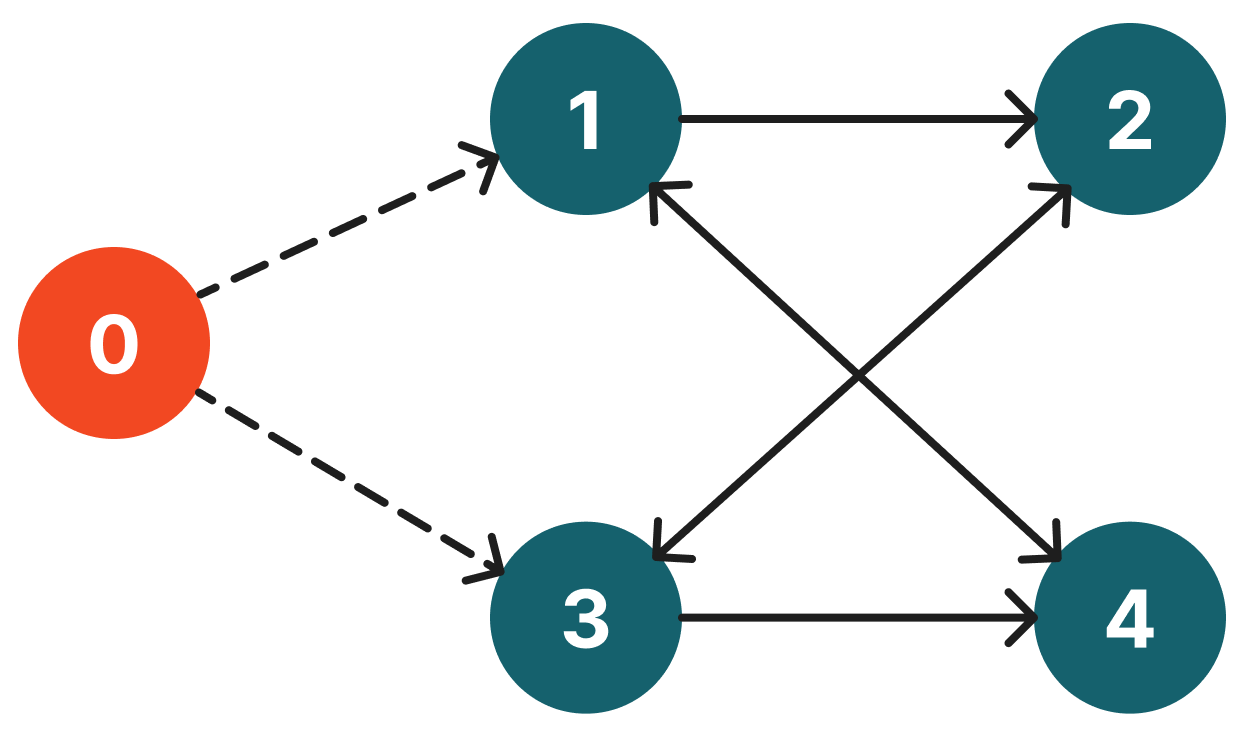
\includegraphics[width=0.45\textwidth]{communication.png}
    \caption{Communication topology among agents.}
    \label{fig:communication1} % Label for referencing the figure
\end{figure}



% \section{Extension to Switching Topology}

% In this section, the proposed design is extendend to the multiagent system with switching topology.

% Let \(\mathcal{G}\) denote a time-varying graph depend on \(k\). The adjacency matrix associated with \(\mathcal{G}(k)\) is denoted by \(\mathcal{A}(k) = (a_{i,j}(k)) \varepsilon R^{N \times N} \) and the Laplacian of \(\mathcal{G}(k)\) is denoted by \(L(k)\). The neighborhood of the \(i\)th agent is denoted by the set \(N_i(k)\). To describe the switching topology, let \(\mathcal{G}_\varrho  =\mathcal{G}_1, \mathcal{G}_2, \dots ,\mathcal{G}_M \) denote the set of all directed graphs for the agents, where \(M \varepsilon Z^+\) denotes the total number of possible interaction graphs. The Laplacian of \(\mathcal{G}_l\) is denoted by \(L-l\) for \(l = 1,2, \dots, M\). We also view the disired trajectory as a virtual leader and, index it by the vertex 0 in the graph representation. In this case, the complete information flow of the whole interation topology can be described as \( \bar{\mathcal{G}}(k)\). 
% In addition \(\bar{\mathcal{G}}_\varrho  =\bar{\mathcal{G}}_1 , \bar{\mathcal{G}}_2 , \dots ,\bar{\mathcal{G}}_M  \) denotes the set of the finite possible interaction graphs for \(\bar{\mathcal{G}}(k)\).
% In this cas, the equation (\ref{model 3}) becomes:
% \begin{equation}
%     \label{model 41}
%     \xi_i(k) = \sum_{j \in N_i(k)} a_i,_j(k)( y_j(k)-y_i(k)) + d_i(k)(yd(k) - y_i(k ))
% \end{equation}

% Assumption 5: The communication graph \(\bar{\mathcal{G}}_l\) is a fixed strongly connected graph and at least one of the follower agents can access the leader's trajectory for all \(l = 1,2,\dots,M\).

% Theorem (?):Consider that the multiagent system (\ref{model 1}) satisfies Assumptios 1,2,3  and communication graph assumption 4. Let the proposed MFAC algorith be used. Assume that the desired trajectory \(y_d(k)\) is time invariable, that is \(yd(k) = const \). If we select \(\rho\) such that it satisfies the condition
% \[
%     \rho < \frac{1}{max_{i=1,2,\dots,N,l=1,2,\dots,M}\sum_{j=1}^{N}a_{i,j}^l + d_i^l}
% \]

% where \(a_{i,j}^l\) is the element of \(L_1\) and \(d_i^l\) is the element of \(D_l\). Then there exists a \(\lambda_min > 0 and \lambda > \lambda_min\) such that the tracking errors \(e_i(k)\) converge to 0 as \(k \rightarrow \infty\) for all \(i = 1,2,\dots, N\). so:

% \[
%     \xi_i(k)  = (L(k) + D(k))e(k)
% \]

% Remark 9: From Theorem 4, we can observe that, it is possible to derive consensus tracking for multiagent systems with
% a time invariable desired trajectory, although the interaction
% graph between agents is time varying. Similarly, the tracking
% results for a time varying desired trajectory can also be given
% by following the result of Theorem 3, which has been omitted
% here.
% Remark 10: From Theorems 2 and 3, we can conclude that
% the distributed MFAC has several attractive properties. First,
% distributed MFAC uses only the real time measurement I/O
% data of the each agent. No mathematical model of the agent’s
% dynamic is needed, which implies that we can develop a
% generic consensus control algorithm for a certain class of multiagent systems. Second, distributed MFAC does not require
% any training process and external testing signals, which are
% necessary for NN-based nonlinear adaptive consensus tracking
% control approaches. Third, since the agent’s dynamic model
% information does not include in the distributed MFAC scheme,
% and then it has strong robustness for traditional unmodeled
% dynamics comparing with the other model based consensus
% control methods. Finally, the distributed MFAC is simple and
% easily implemented with small computational cost.

\section{Simulation Example}



% Assumption 5: The communication graph \(\bar{\mathcal{G}}_l\) is a fixed strongly connected graph and at least one of the follower agents can access the leader trajectory for all \(l = 1,2,\dots,M\).


% This section describes the methodology and hardware used for speed regulation, including the calculation of motor speed using the quadruple-frequency data processing  method and .


% The DC brushed motors have a rated voltage of 12V, an unloaded speed of 293 ± 21 RPM and a rated current of 0.36 A. The gear ratio of 20 means that the output speed of the motor is 1/20 of the rotor speed, resulting in higher torque with a higher gear ratio. The Hall encoders used have 13 pulses per revolution, meaning each full rotation generates 13 pulse signals. 

% To enhance measurement accuracy, employing the quadruple-frequency data processing method. This technique quadruples the effective resolution of the encoder by processing the output pulse signals at four times the frequency, thus increasing measurement precision by a factor of four.

% \subsection{Data Processing Method}

This section describes the usefulness of the provided control approach, which is validated by numerical simulations and physical experiments results. 

The motor speed is measured in revolution per second $(r/s)$ based on encoder measurements and the sampling interval $t$. The total number of encoder counts per revolution is calculated as $ rT=4N_{e}R{r} $, where $N_e$ is the encoder line count equal to 13, $R_r$ is the reduction ratio equal to 20 and the factor of 4 accounts for quadrature encoding. The number of rotations, $N_r$ is determined using $N_r = \frac{m}{rT}$, with $m$ representing the total encoder count. The output data model of each agent is governed by:

% The speed of the motor is then derived as:

% \begin{equation}
%            \label{motor_speed}
%            v = \frac{N_r}{t} = \frac{m}{T  t}
% \end{equation}


% The quadruple-frequency method is crucial for maximizing encoder measurement precision, resulting in more accurate speed control for the motor system.


% \[
% \begin{array}{c}
% \text{Agent 1}: \quad y_1(k+1) = 0.5 * y_1(k) * u_1(k) + 1.2 * \frac{m}{(rT * 0.2)} - 0.03 * y_1(k)^3 + 0.45\\
% \text{Agent 2}: \quad y_2(k+1) = 0.5 * y_2(k) * u_2(k) + 1.2 * \frac{m}{(rT * 0.2)} - 0.01 * y_2(k)^2 + 0.45\\
% \text{Agent 3}: \quad y_3(k+1) = 0.5 * y_3(k) * u_3(k) + 1.2 * \frac{m}{(rT * 0.2)} - 0.02 * y_3(k)^3 + 0.45\\
% \text{Agent 4}: \quad y_4(k+1) = 0.5 * y_4(k) * u_4(k) + 1.2 * \frac{m}{(rT * 0.2)} - 0.01 * y_4(k)^2 + 0.45\\
% \end{array}
% \]
\[
y_i(k+1) = 0.5 y_i(k) u_i(k) + \frac{6m}{rT} - a_i y_i(k)^{p_i} + 0.45, \quad i = 1, 2, 3, 4,
\]
where the agent-specific parameters are:
\[
a_i = \begin{cases} 
0.03 & \text{if } i=1 \\
0.01 & \text{if } i=2 \\
0.02 & \text{if } i=3 \\
0.01 & \text{if } i=4
\end{cases}
\qquad
p_i = \begin{cases} 
3 & \text{if } i=1, 3 \\
2 & \text{if } i=2, 4
\end{cases}
\]

in this scenario, noting that the four agents have different dynamics, the parameters \(a_i\) and \(p_i\) are set to different values for each agent. In addition, they are given only to generate the I/O data for the MASs. 

As illustrated in Fig. 2, the virtual leader is designated as vertex 0. It can be observed that only agents 1 and 3 can receive information from the leader, forming a strongly connected communication graph. The Laplacian matrix of the graph is given as follows:

\[
    L = \begin{bmatrix}
    1 & 0 & 0 & -1 \\
    -1 & 2 & -1 & 0 \\
    0 & -1 & 1 & 0 \\
    -1 & 0 & -1 & 2
    \end{bmatrix}
\]
with \( D = \text{diag}(1, 0, 1, 0) \), the following two different reference trajectories are introduced to demonstrate the effectiveness of the proposed method.



Example 1: Consider the following reference trajectory:

% \[
% y_d(k) = 0.5 \sin\left(\frac{k \pi}{30}\right) + 0.3  \cos\left(\frac{k \pi}{10}\right)
% \]

$ y_d(k) = 0.6, k \in [0, 200]  $



The initial parameters are chosen as \(u_i(1)=0.01\), \(y_i(1)=0.6\) and \(\phi_i(0)=4 \) for all agents in this simulation, \(\Gamma_{1}=\Gamma_{3}=0.45\) and \(\Gamma_{2}=\Gamma_{4}=0.15\), with \(\tau_s=10^{-5}\), \(m=200\), sampling rate $rT = 1024 $, \(\eta=1\), \(\mu=0.005\), other parameters are given as \(\rho=7.5\), \(\lambda=350\), $ \omega = 10 $, $ \sigma=95 $, \(\alpha=15\) with \(\epsilon=10^{-5}\).
\begin{figure}[H]
    \centering
    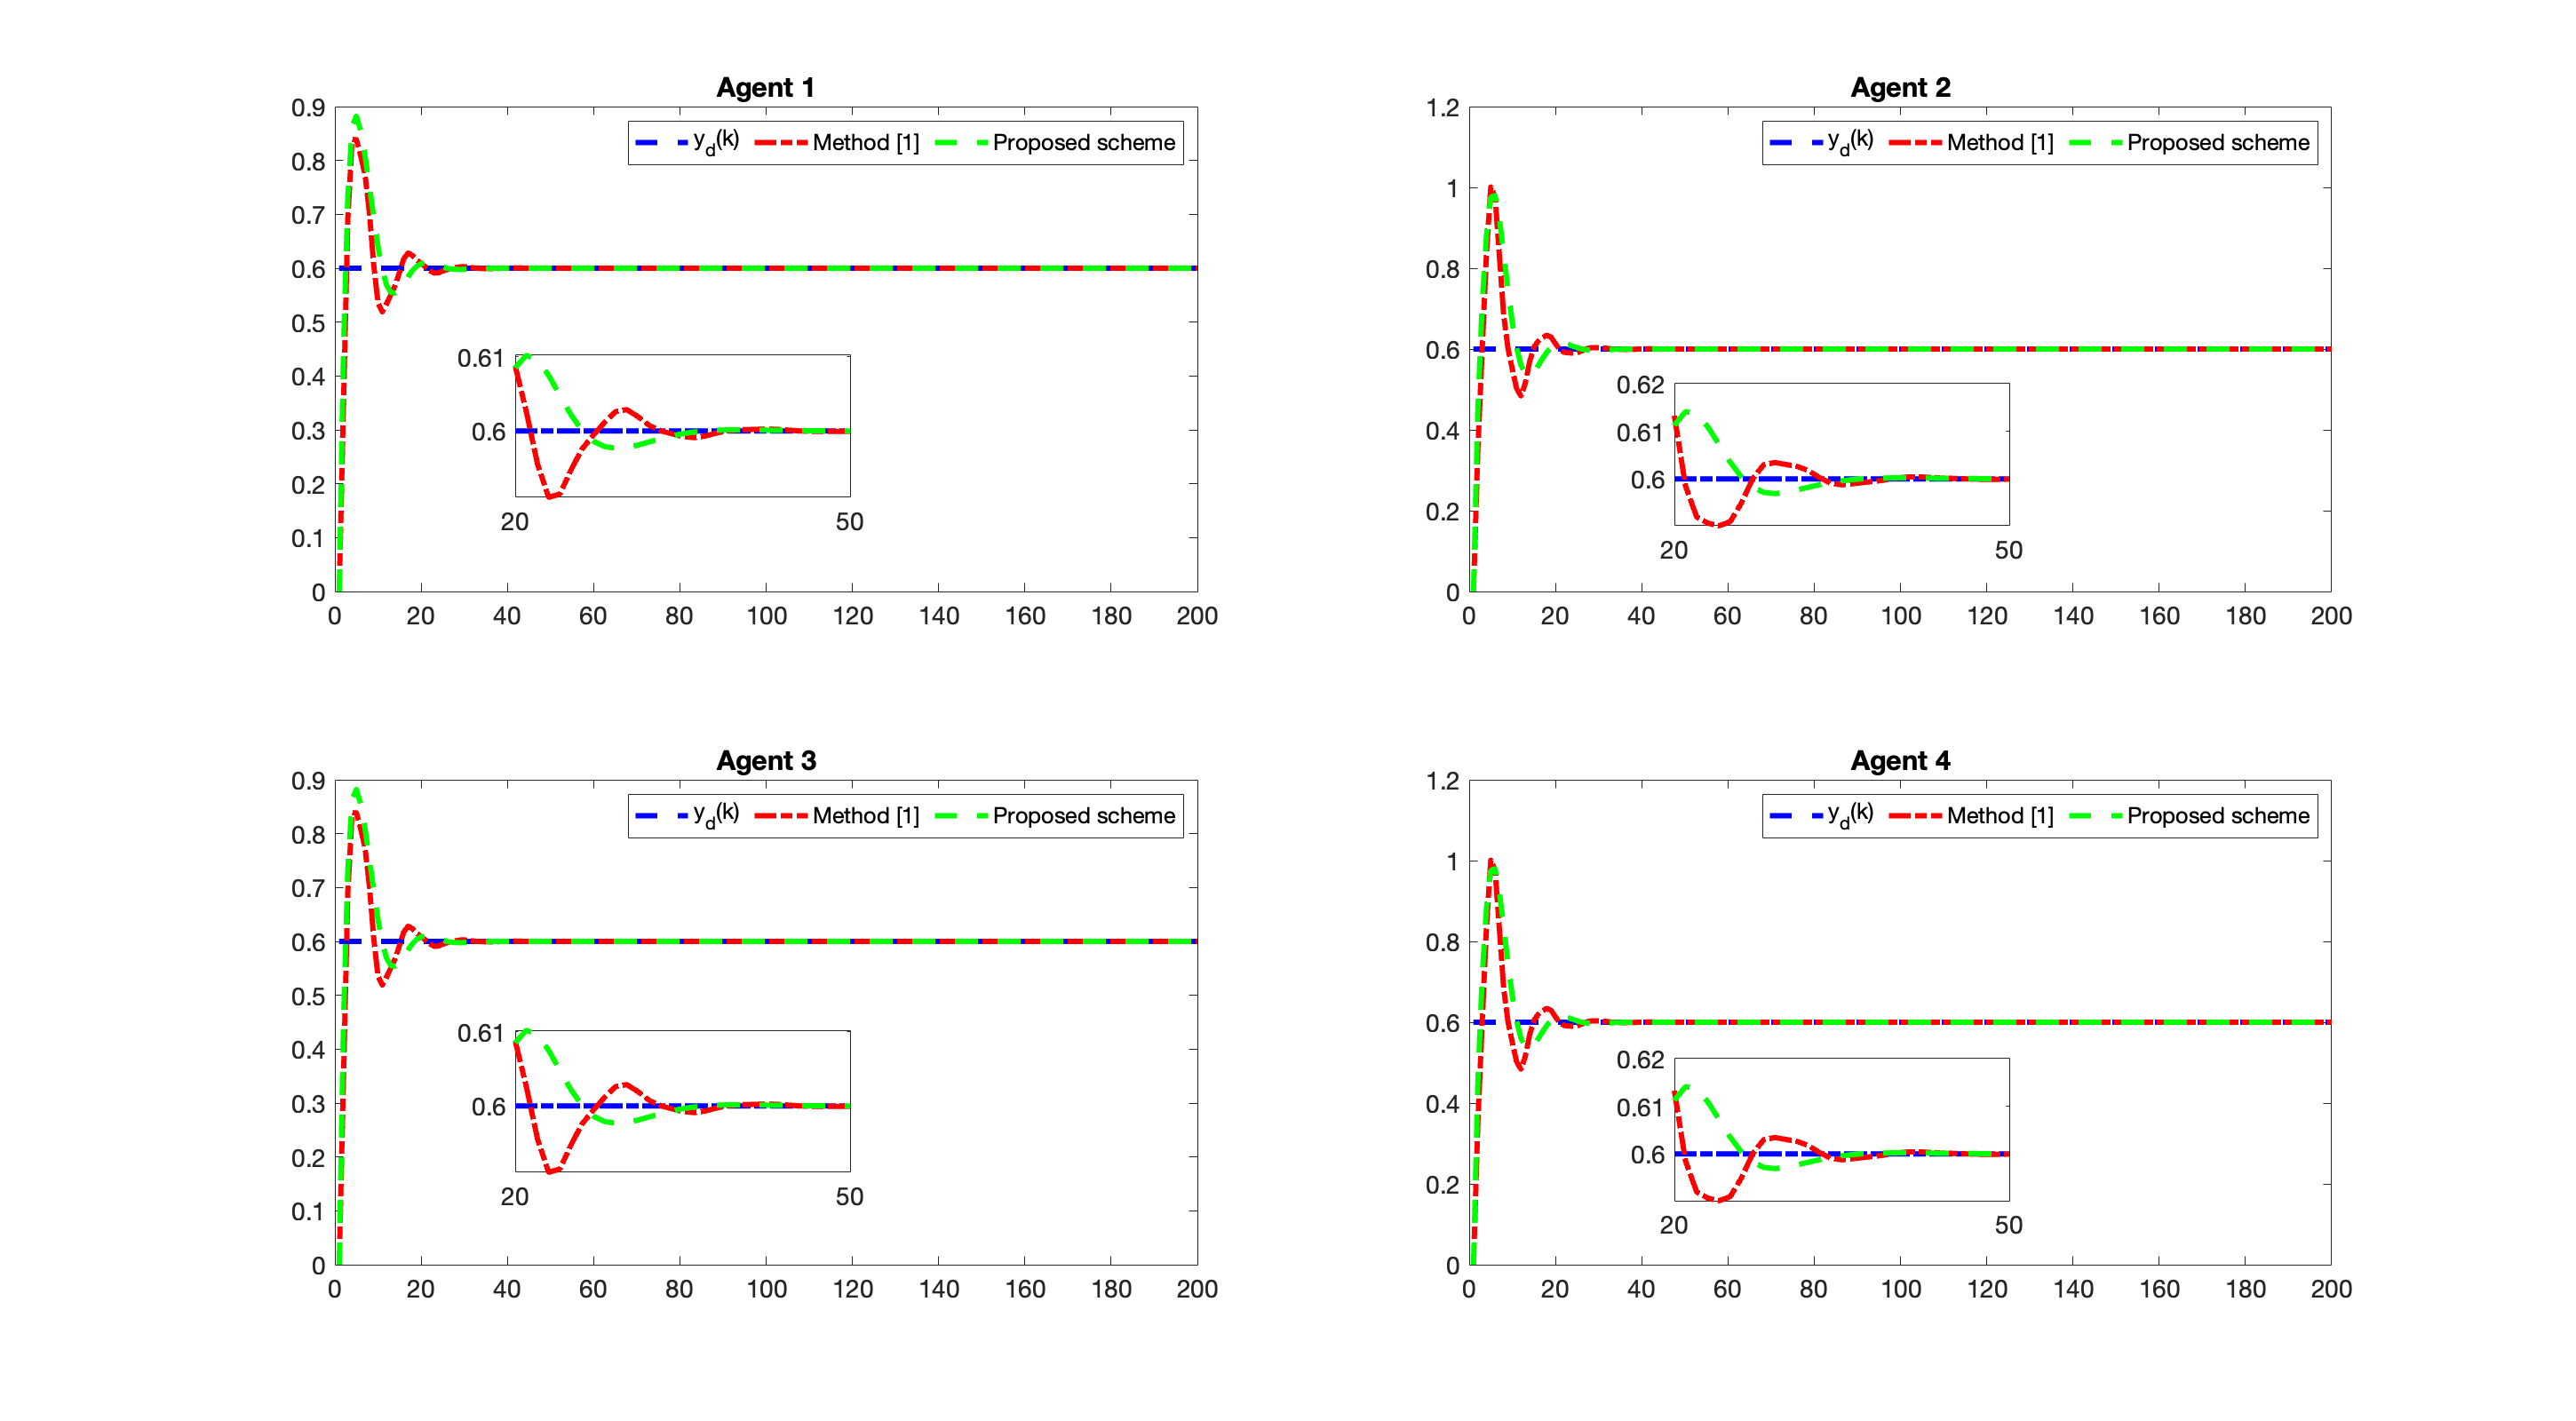
\includegraphics[width=0.9 \textwidth]{inv_tracking.png}
    \caption{Tracking performance of all agents under the time-invarying reference trajectory.}
    \label{fig:tracking_inv} % Label for referencing the figure
\end{figure}


Fig.~\ref{fig:tracking_inv} demonstrates the tracking output of the proposed control scheme for the case of a time-invariant reference signal. It can be clearly observed that the agents effectively follow the reference trajectory, which is set to a constant value of 0.6, and the tracking performance closely aligns with this target. 

\clearpage
Moreover, Fig.~\ref{fig:error_inv} illustrates the corresponding distributed measurement error, which remains bounded within the range of [-0.01, 0.01], indicating accuracy of the control strategy. These results confirm that the controller maintains stability.


\begin{figure}[H]
    \centering
    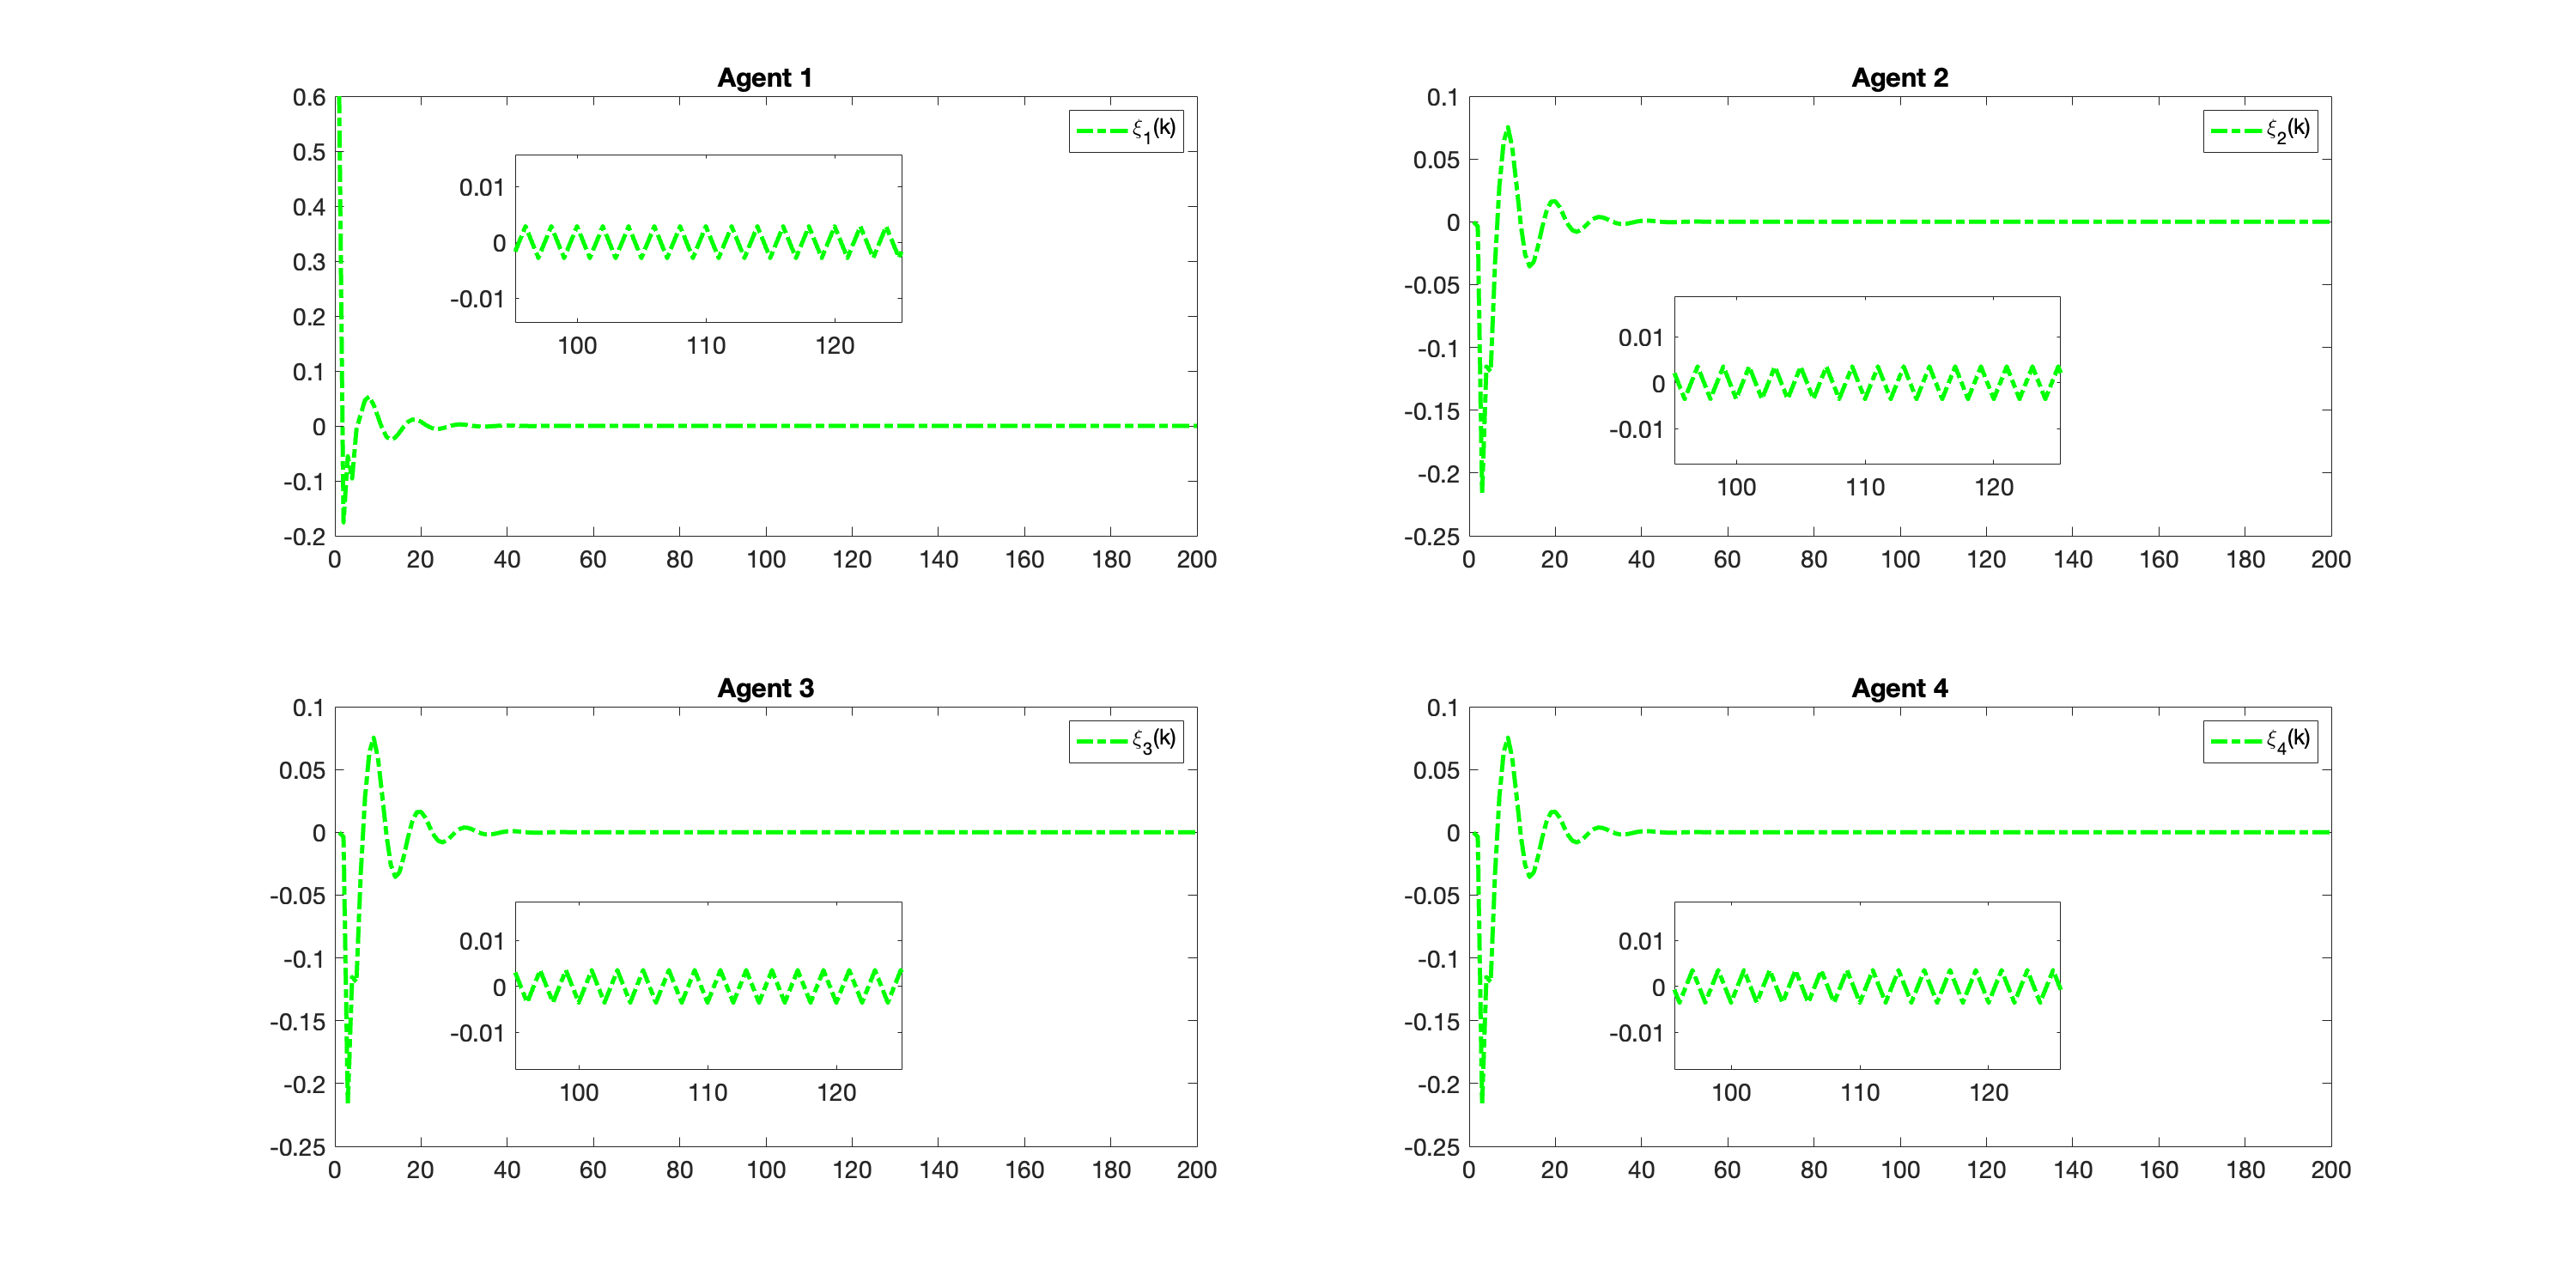
\includegraphics[width=0.9 \textwidth]{inv_error.png}
    \caption{Distributed measurement error of all agents under the time-invarying reference trajectory.}
    \label{fig:error_inv} % Label for referencing the figure
\end{figure}


Example 2: The expression for the reference trajectory is:
\[ y_d(k)=0.6\sin(0.07\pi(k))+0.6\cos(0.04\pi(k)), k \in [0, 200] \]

\begin{figure}[H]
    \centering
    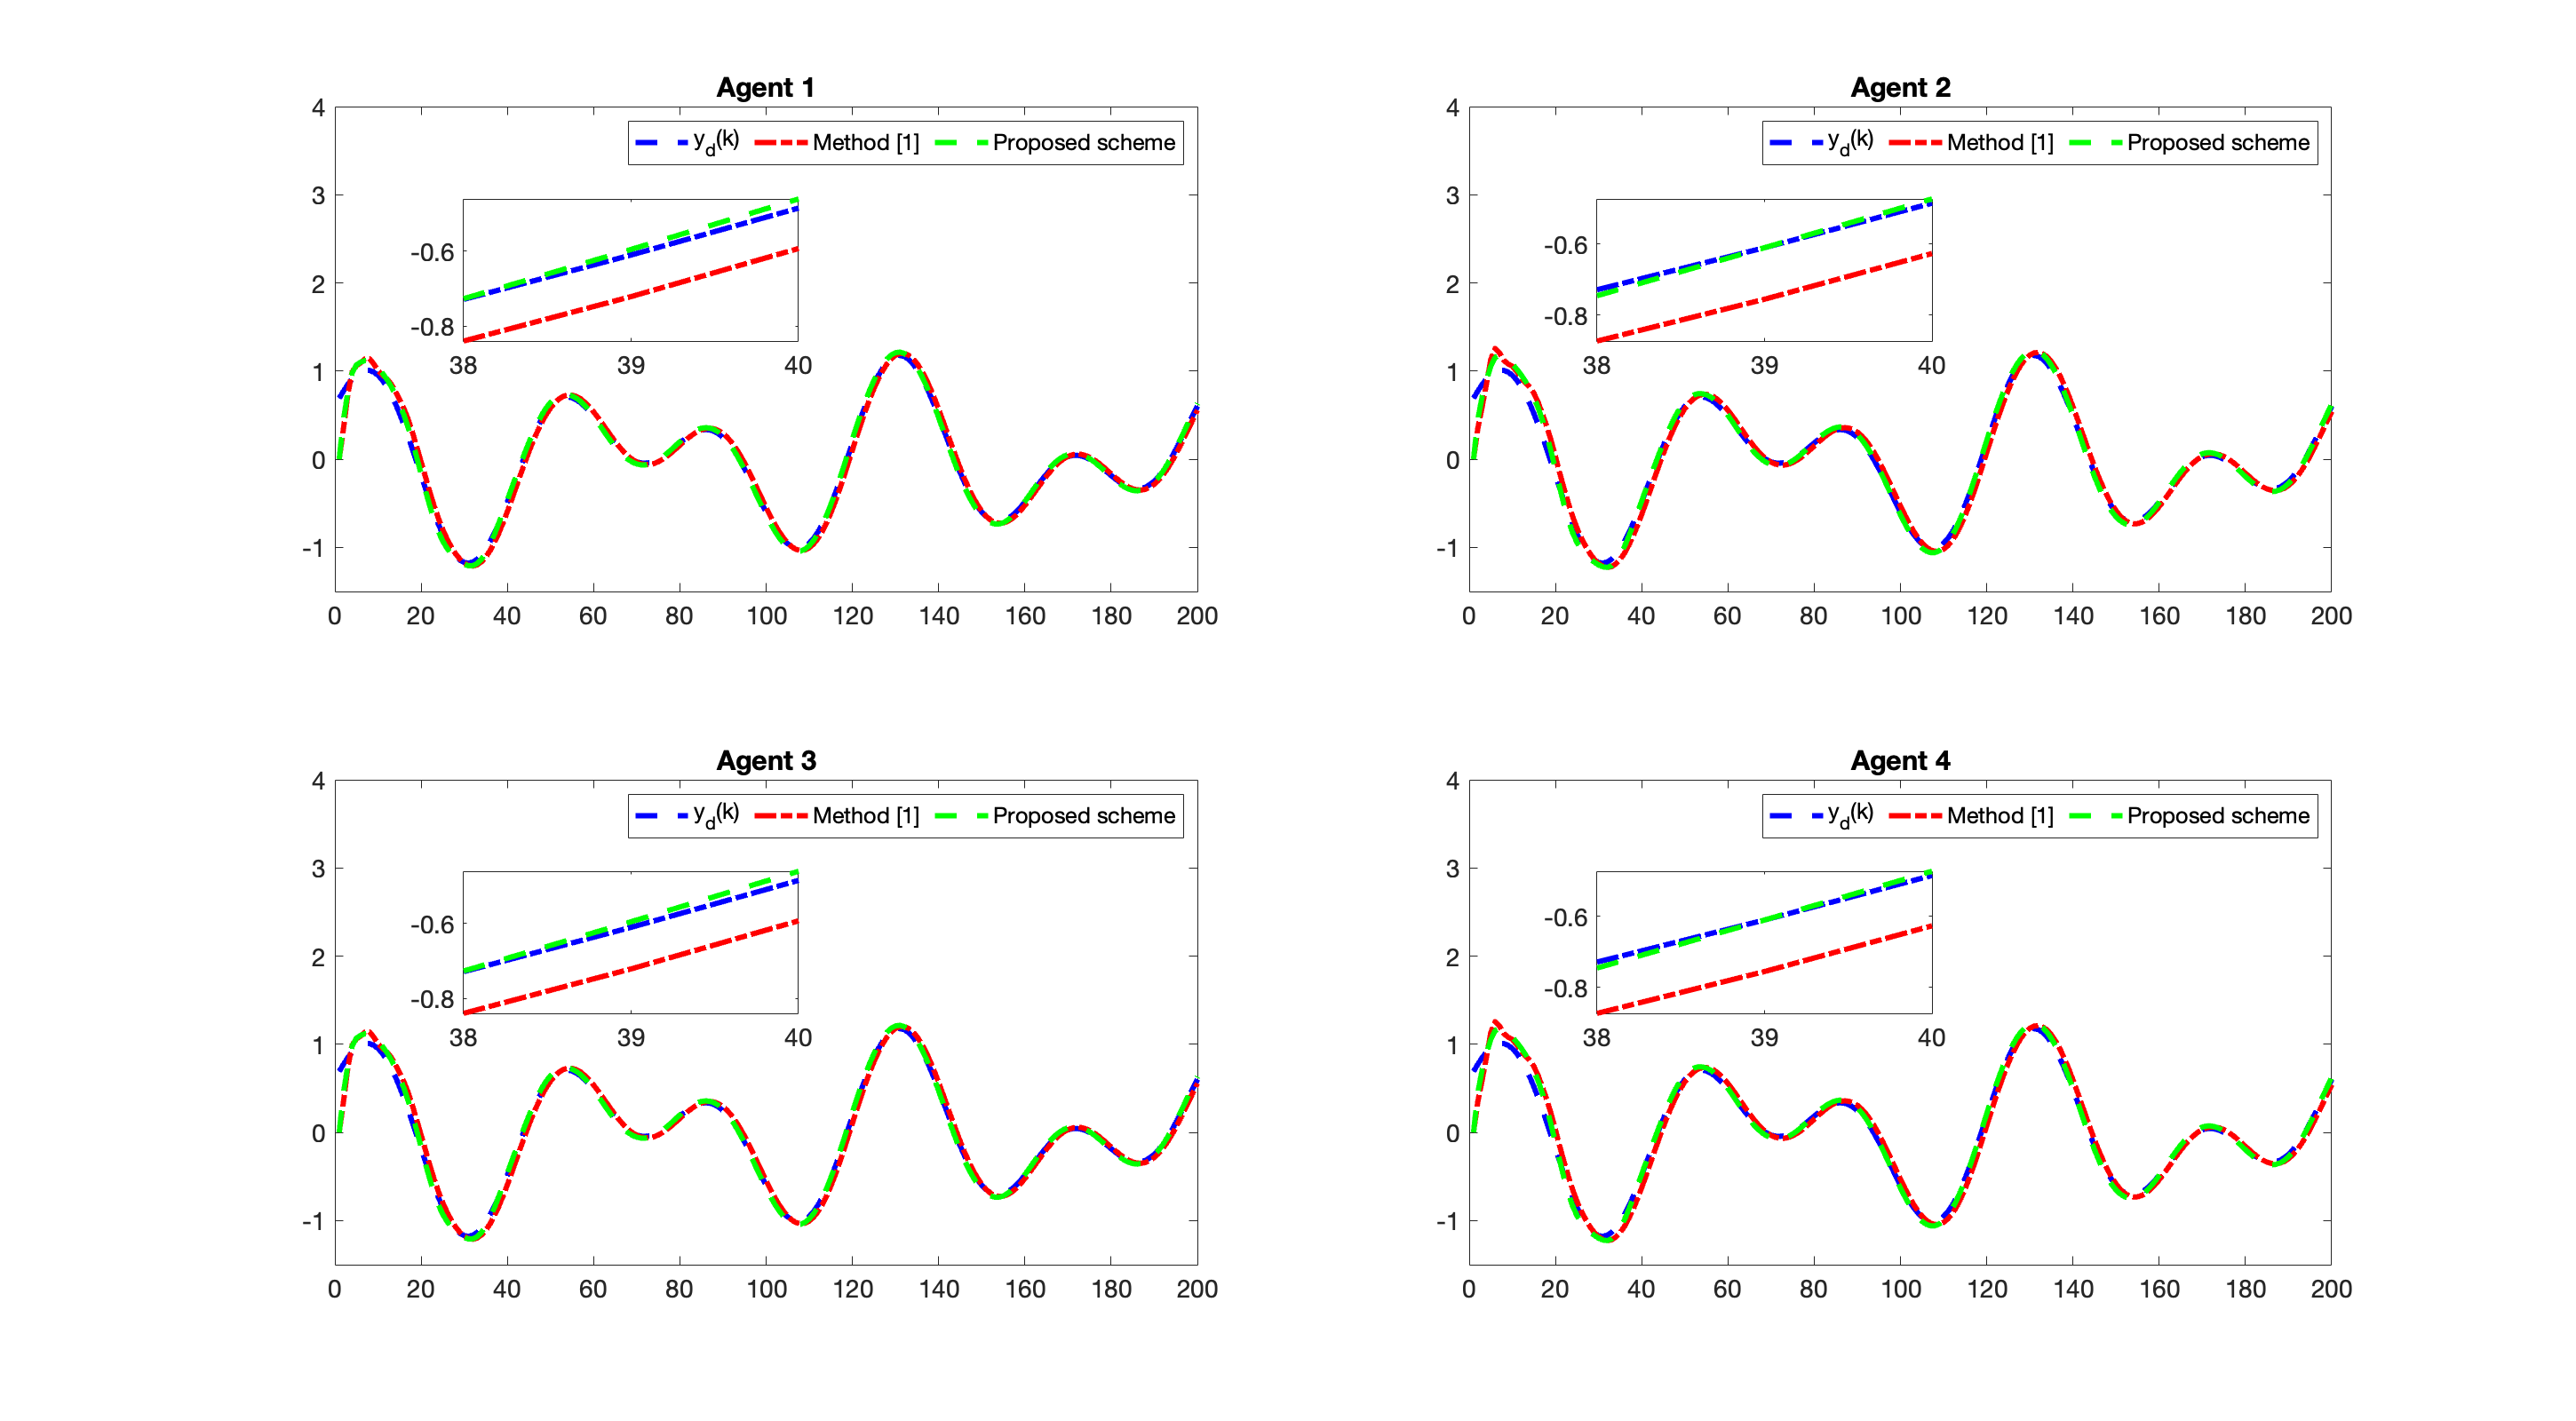
\includegraphics[width=0.9\textwidth]{var_tracking.png}
    \caption{Tracking performance of all agents under the time-varying reference trajectory.}
    \label{fig:tracking_var} % Label for referencing the figure
\end{figure}


\begin{figure}[H]
    \centering
    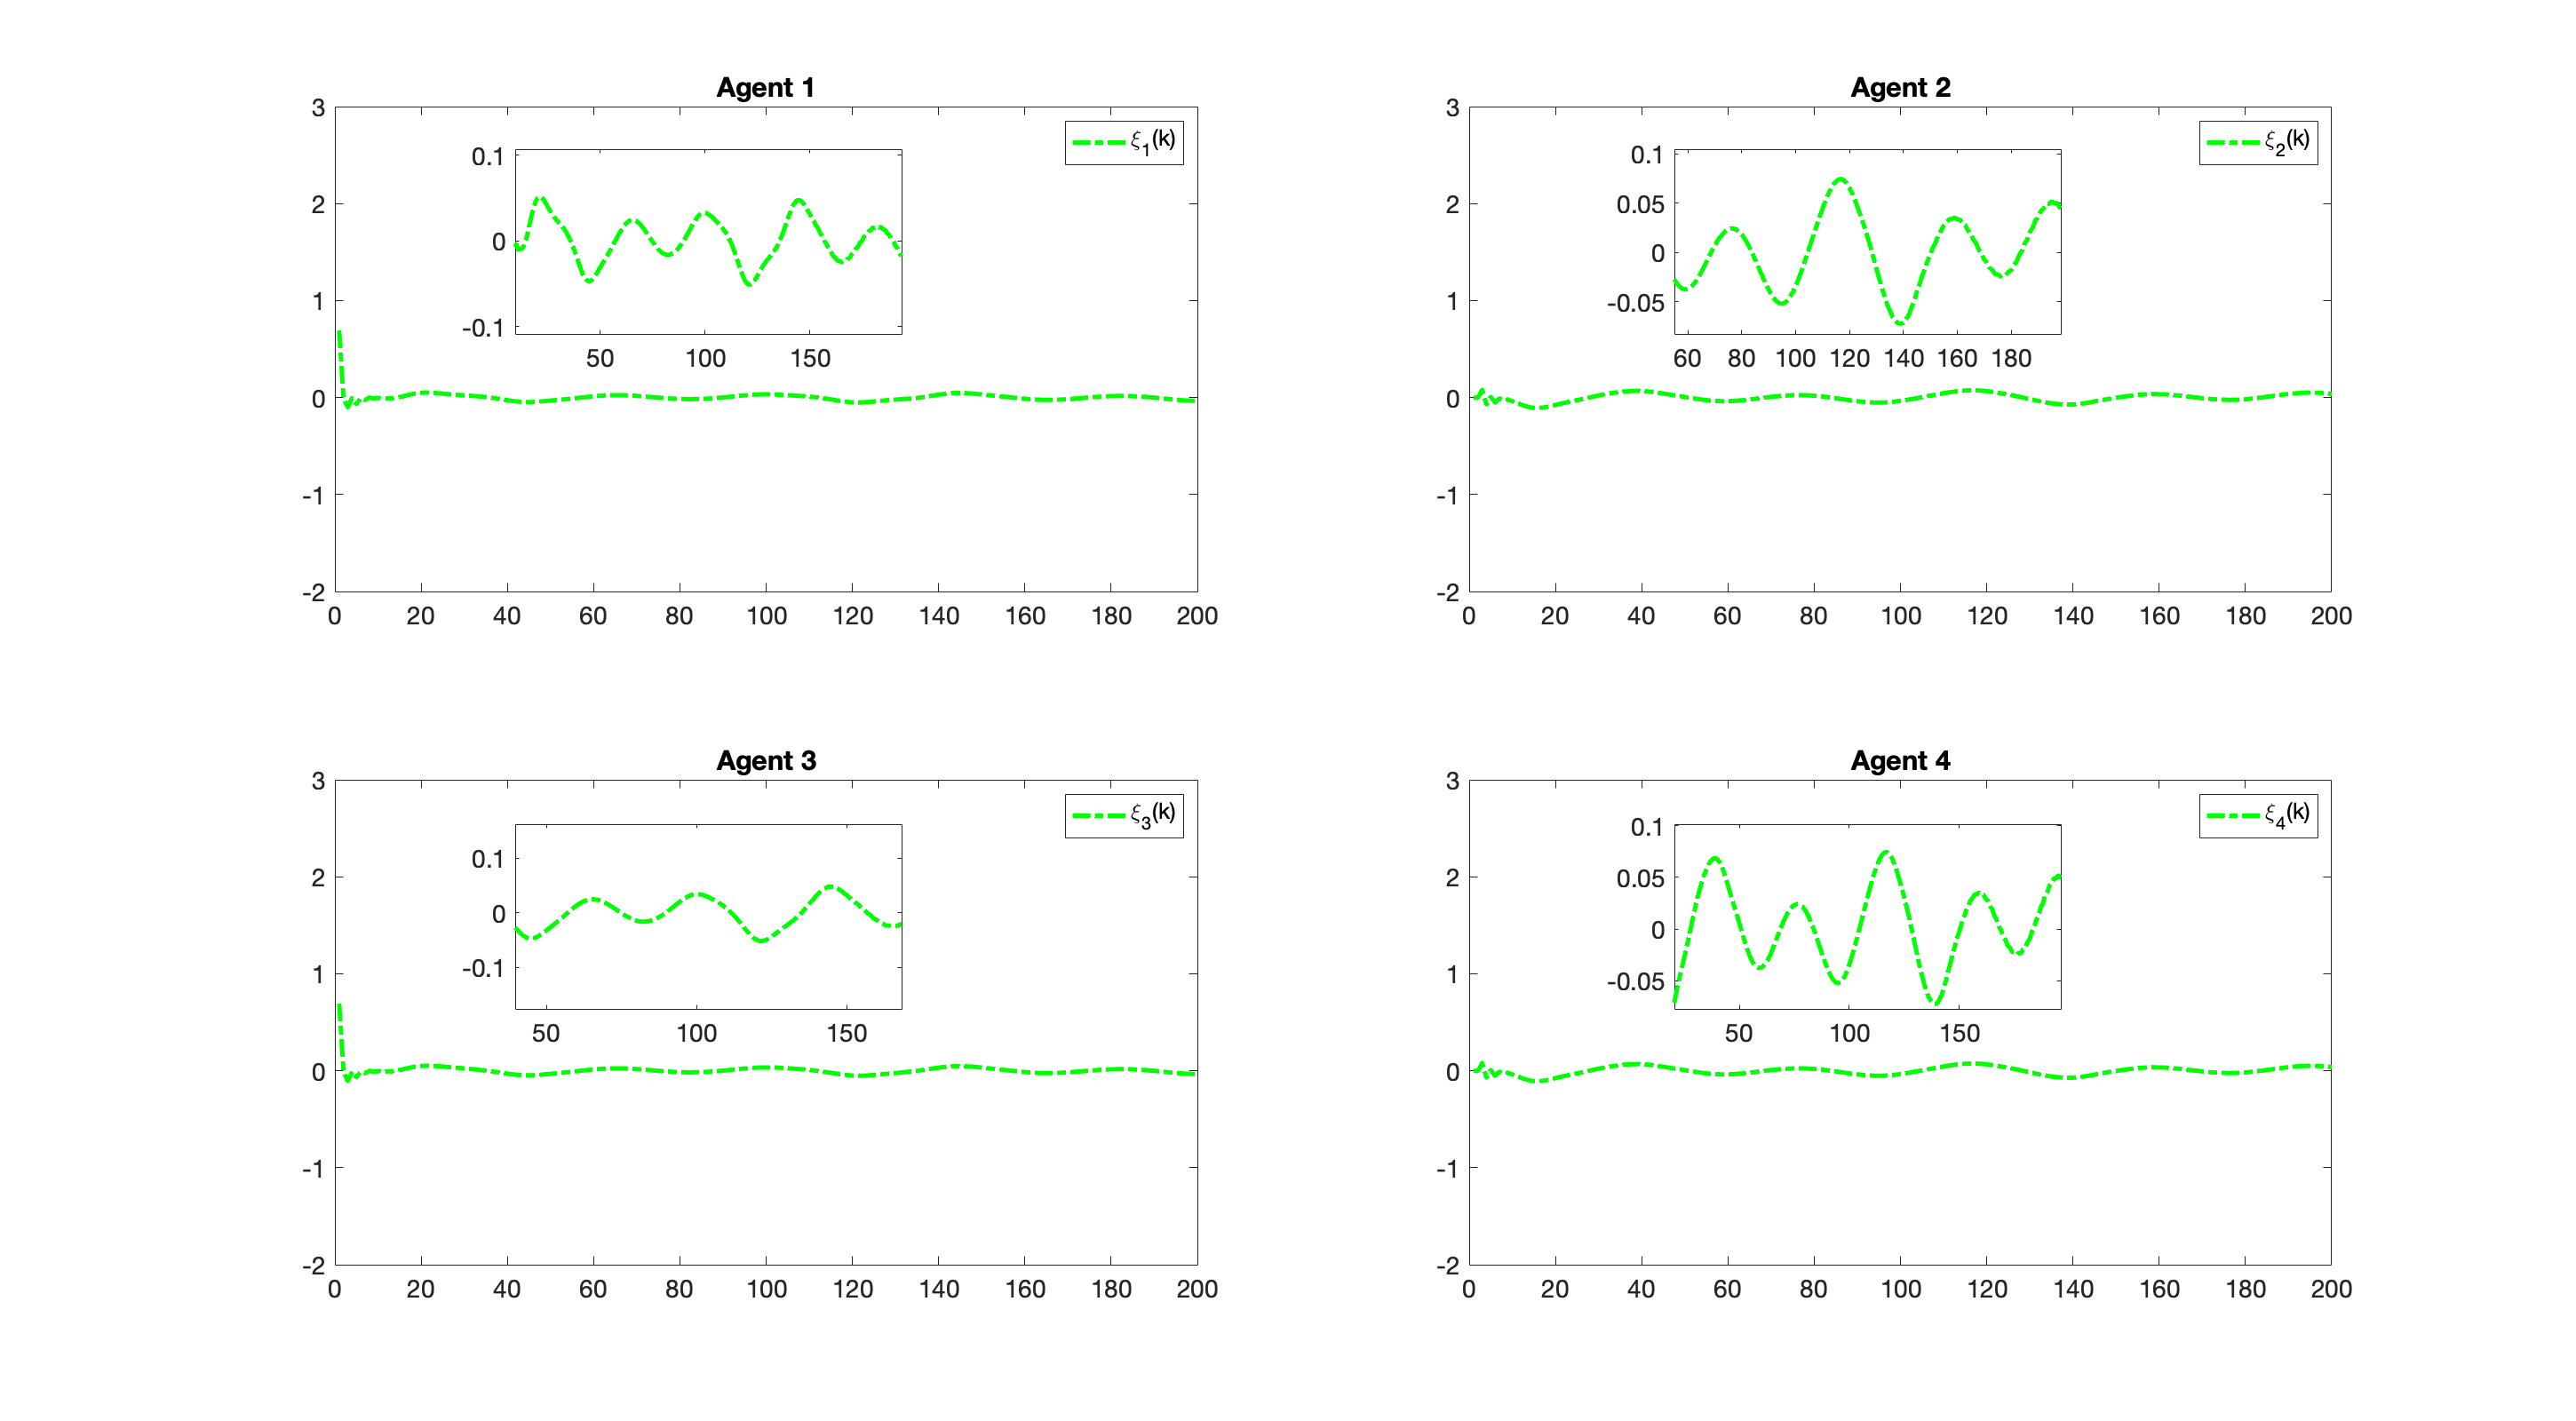
\includegraphics[width=0.9\textwidth]{var_error.png}
    \caption{Distributed measurement error of all agents under the time-varying reference trajectory.}
    \label{fig:error_var} % Label for referencing the figure
\end{figure}

Fig. \ref{fig:tracking_var} presents the tracking performance for all agents for the time-varying trajectory. All agents successfully track the time-varying reference trajectory. Additionally, as shown in Fig. \ref{fig:error_var}, the distributed measurement errors of all agents are bounded within a specified range 

\begin{figure}[H]
    \centering
    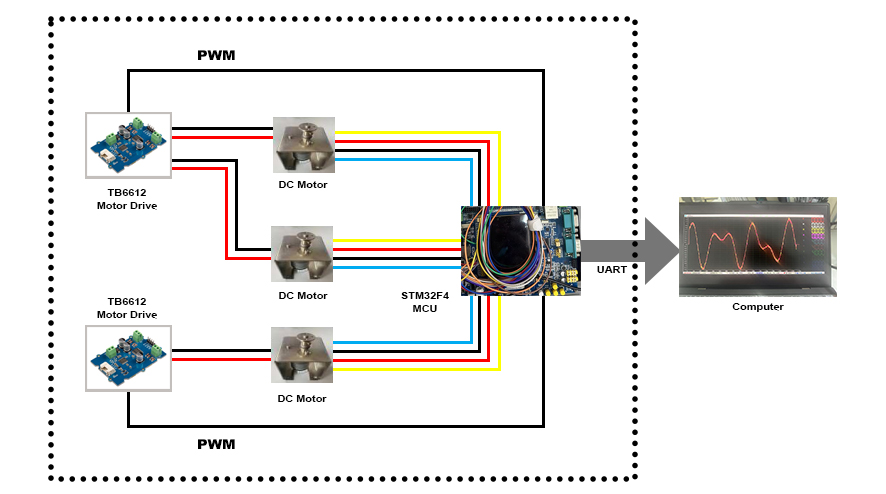
\includegraphics[width=0.75\textwidth]{diagram.jpg}
    \caption{System connection diagram of multi DC motor consensus tracking control.}
    \label{fig:system_diagram} % Label for referencing the figure
\end{figure}

To verify the proposed consensus tracking control methodology, the experimental validation is conducted using a multi DC motor system, as illustrated in Fig. \ref{fig:system}. The system consists of three DC motors equipped with Hall encoders and reduction
gears, an STM32F407 main control chip, two motor drive modules, and an LCD display module. The microcontroller unit (MCU) STM32F407ZGT6 is used for high-resolution pulse width modulation (PWM) output generation to achieve precise motor speed control. The timer module is utilized for this purpose.

In addition, the controller code is written in C language using STM32CubeIDE, while STM32CubeMX is used for pin configuration. The main purpose of the experiment is to ensure that the three motors accurately track the reference trajectory:
% \[ y_d(k)=0.5\sin(0.07\pi(k))+0.7\cos(0.04\pi(k)) \]

\begin{figure}[H]
    \centering
    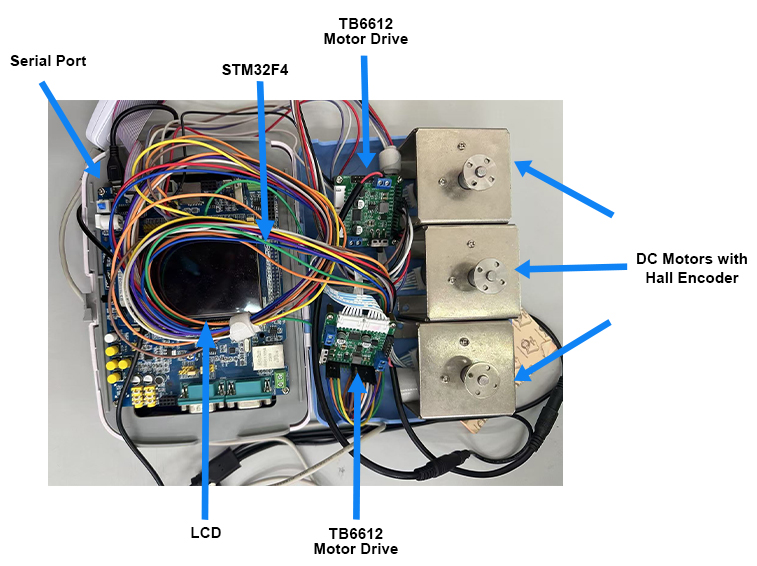
\includegraphics[width=0.65\textwidth]{system.jpg}
    \caption{Multi DC motor system.}
    \label{fig:system} % Label for referencing the figure
\end{figure}


\begin{figure}[H]
    \centering
    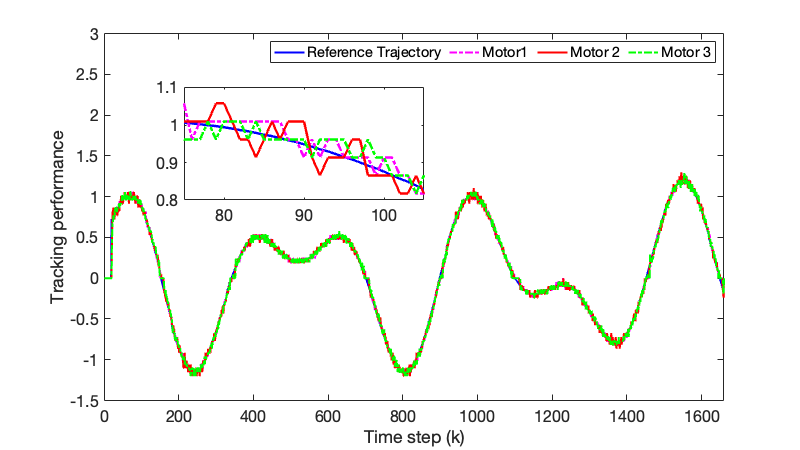
\includegraphics[width=0.9\textwidth]{dataplot.png}
    \caption{Tracking performance of 3 DC motors for time-invariable desired trajectory.}
    \label{fig:output} % Label for referencing the figure
\end{figure}

Fig. \ref{fig:output} shows the tracking performance of multi DC motor demonstrating the effectiveness of the proposed control method.
Overall, the simulation results suggest that the proposed control system is capable of tracking a constant desired trajectory for multiple agents. While initial transient errors may accur, the system eventually reaches a steady-state condition with minimal tracking error. The variations in tracking performance among the agents highlight the potential influence of individual characteristics and external factors.

\section{Conclusion}

In this study, the model-free adaptive sliding mode control approach is presented to address the consensus problem of MASs. Firstly, the equivalent data model for each agent is obtained using the CFDL method. Secondly, a novel sliding surface ireas presented to ensure that the distributed measurement error remains bounded. Finally, the effectiveness of the proposed control approach is verified through physical experiments on multi DC motor system.




% \begin{thebibliography}{99}
%     \bibitem{1}
%     Bu, XH; Hou, ZS and Zhang, HW. Data-Driven Multiagent Systems Consensus Tracking Using Model Free Adaptive Control.{\sl 
%     IEEE TRANSACTIONS ON NEURAL NETWORKS AND LEARNING SYSTEMS}, May 2018,29{\bf (5)}: 1514-1524.

%     \

%     \bibitem{2}

%     \

% \end{thebibliography}

\begin{thebibliography}{99}


    \bibitem{1}
    X. Bu, Z. Hou, and H. Zhang, “Data-driven multiagentsystems consensus tracking using model free adaptive control,” IEEE Transactions on Neural Networks and Learning
    Systems, vol. 29, no. 5, pp. 1514-1524, 2018.
    
    \bibitem{2}
    M. Parsa and M. Danesh, “Robust containment control of uncertain multi-agent systems with time-delay and heterogeneous lipschitz nonlinearity,” IEEE Transactions on Systems, Man, and Cybernetics: Systems, vol. 51, no. 4, pp.
    2312-2321, 2021.

    \bibitem{3}
    A.-Y. Lu and G.-H. Yang, “Distributed secure state estimation for linear systems against malicious agents throughsorting and filtering,” Automatica, vol. 151, pp. 110927,2023.

    \bibitem{4}
    T. Li, W. Bai, Q. Liu, Y. Long and C. L. P. Chen, “Distributed fault tolerant containment control protocols for the discrete-time multiagent systems via reinforcement learning method,” IEEE Transactions on Neural Networks and Learning Systems, vol. 34, no. 8, pp. 3979-3991, Aug. 2023
    
    \bibitem{5}
    Y. Yang, Y. Xiao and T. Li, “Attacks on formation control for multiagent
    systems,” IEEE Transactions on Cybernetics, vol. 52, no. 12, pp. 12805-
    12817, Dec. 2022
    
    \bibitem{6}
    R. Olfati-Saber, J. A. Fax, and R. M. Murray, "Consensus and cooperation in networked multi-agent systems," \textit{Proceedings of the IEEE}, vol. 95, no. 1, pp. 215-233, 2007.
    
    \bibitem{7}
    M. Sampei, T. Tamura, T. Kobayashi, and N. Shibui, “Arbitrary path
    tracking control of articulated vehicles using nonlinear control theory,”
    IEEE Trans. Control Syst. Technol., vol. 3, no. 1, pp. 125–131, Mar. 1995.
    
    \bibitem{8}
    W. Ren, R. W. Beard, and E. M. Atkins, "Information consensus in multivehicle cooperative control," \textit{IEEE Control Systems}, vol. 27, no. 2, pp. 71-82, 2007.
    
    \bibitem{9}
    D. Xu, B. Jiang, and P. Shi, "Adaptive observer based data-driven control for nonlinear discrete-time processes," \textit{IEEE Transactions on Automation Science and Engineering}, vol. 11, no. 4, pp. 1037-1045, 2014.
    
    \bibitem{10}
    J. Wang, X. Wang, X. Zhang, and S. Zhu, “Global h-synchronization for high-order delayed inertial neural networks via direct SORS strategy,” \textit{IEEE Transactions on Systems, Man, and Cybernetics: Systems}, vol. 53, no. 11, pp. 6693–6704, 2023.
    
    
    \bibitem{11}
    F. Xu, X. Ruan, and X. Pan, “Event-triggered leaderfollowing consensus control of multiagent systems against DoS attacks,” International Journal of Control, Automation and Systems, vol. 22, pp. 3424-3433, 2024.
    
    \bibitem{12}
    Y. Liu, L. Liu, and S. Tong, “Adaptive neural network tracking design for a class of uncertain nonlinear discrete time systems with dead-zone,” Science China Information
    Sciences, vol. 57, pp. 1-12, 2014.
    
    \bibitem{13}
    Z. Dong, X. Wang, X. Zhang, M. Hu, and T.N. Dinh, “Global exponential synchronization of discrete-time high order switched neural networks and its application to multi channel audio encryption,” Nonlinear Analysis: Hybrid
    systems, vol. 47, pp. 101291, 2023.
    
    \bibitem{14}
    X. Liu, J. Lam, W. Yu, and G. Chen, "Finite-time consensus of multiagent systems with a switching protocol," \emph{IEEE Transactions on Neural Networks and Learning Systems}, vol. 27, no. 4, pp. 853–862, Apr. 2016.

    \bibitem{15}
    Z. Hou and Z. Wang, “From model-based control to data-driven control:
    Survey, classification and perspective,” Inf. Sci., vol. 235, pp. 3–35, 2013.

    \bibitem{16}
    Z. Hou and S. Jin, “A novel data-driven control approach for a class
    of discrete-time nonlinear systems,” IEEE Trans. Control Syst. Technol.,
    vol. 19, no. 6, pp. 1549–1558, Nov. 2011.

    \bibitem{17}
    Y. Asadi, M.M. Farsangi, and M.H. Rezaei, “Improved data-driven adaptive control structure against input and output saturation,” International Journal of Control, Automation and Systems, vol. 22, pp. 2981-2989, 2024.

    \bibitem{18}
    Y. Hui, R. Chi, B. Huang, Z. Hou, and S. Jin, “Observer-based sampled-data model-free adaptive control for continuous-time nonlinear nonaffine systems with input rate constraints,” IEEE Transactions on Systems, Man, and Cybernetics: Systems, vol. 51, no. 12, pp. 7813-7822, 2021.

    \bibitem{19}
    Y.-S. Ma, W.-W. Che, C. Deng, and Z.-G. Wu, “Distributed model-free adaptive control for learning nonlinear MASs under DoS attacks,” IEEE Transactions on Neural Networks and Learning Systems, vol. 34, no. 3, pp. 1146-1155, 2023.

    \bibitem{20}
    H. Wang, Q. Luo, N. Li, and W. Zheng, “Data-driven model free formation control for multi-USV system in complex marine environments,” International Journal of Control,
    Automation and Systems, vol. 20, pp. 3666-3677, 2022.

    \bibitem{21}
    L. Duan, Z. Hou, X. Yu, S. Jin, and K. Lu, “Data-driven model-free adaptive attitude control approach for launch vehicle with virtual reference feedback parameters tuning method,” IEEE Access, vol. 7, pp. 54106-54116, 2019.

    \bibitem{22}
    Kiam Heong Ang, G. Chong and Yun Li, “PID control system analysis, design, technology,” IEEE Transactions on Control Systems Technology, vol. 13, no. 4, pp. 559-576, Jul. 2005.
    
    \bibitem{23}
    P. Zhu, S. Jin, X. Bu and Z. Hou, “Improved model-free adaptive control for MIMO nonlinear systems with event-triggered transmission scheme and quantization,” IEEE Transactions on Cybernetics, vol. 53, no. 9, pp. 5867-5880, Sept. 2023.
    
    \bibitem{24}
    D. Xu, Y. Shi and Z. Ji, “Model-free adaptive discrete-time integral
    sliding-mode-constrained-control for autonomous 4WMV parking systems,” IEEE Transactions on Industrial Electronics, vol. 65, no. 1, pp.
    834-843, Jan. 2018.
    
    \bibitem{25}
    D. Liu and G.-H. Yang, “Prescribed performance model-free adaptive integral sliding mode control for discrete-time nonlinear systems,” IEEE Transactions on Neural Networks and Learning Systems, vol. 30, no. 7, pp. 2222-2230, Jul. 2019.
    
    \bibitem{26}
    P. Shi, Y. Xia, G. Liu, D. Rees, On designing of sliding-mode control for stochastic jump systems, IEEE Trans. Automat. Control 51 (1) (2006) 97–103.
    
    \bibitem{27}
    D. Liu and G.-H. Yang, “Data-driven adaptive sliding mode control of nonlinear discrete-time systems with prescribed performance,” IEEE Transactions on Systems, Man, and Cybernetics: Systems, vol. 49, no. 12, pp. 2598-2604, 2019.
    
    \bibitem{28}
    Z. Wu, X. Wang, and X. Zhao, “Backstepping terminal sliding mode
    control of DFIG for maximal wind energy captured,” Int. J. Innovative
    Comput. Inf. Control, vol. 12, no. 5, pp. 1565–1579, 2016.

    \bibitem{29}
    X. Yan and C. Edwards, “Adaptive sliding-mode-observer-based fault
    reconstruction for nonlinear systems with parametric uncertainties,” IEEE
    Trans. Ind. Electron., vol. 55, no. 11, pp. 4029–4036, Nov. 2008.

    \bibitem{30}
    J. Liu, W. Luo, X. Yang, and L. Wu, “Robust model-based fault diagnosis
    for PEM fuel cell air-feed system,” IEEE Trans. Ind. Electron., vol. 63,
    no. 5, pp. 3261–3270, May 2016.

    \bibitem{31}
    A. Anuchin, A. Dianov and F. Briz, "Synchronous Constant Elapsed Time Speed Estimation Using Incremental Encoders," in IEEE/ASME Transactions on Mechatronics, vol. 24, no. 4, pp. 1893-1901, Aug. 2019, doi: 10.1109/TMECH.2019.2928950.

    \bibitem{32}
    S. Qin and T. Badgwell, “A survey of industrial model predictive control
    technology,” Control Eng. Pract., vol. 11, pp. 733–764, 2003.

    % \bibitem{32}
    % A. Sharafian, V. Bagheri, and W. Zhang, "RBF neural network sliding mode consensus of multi-agent systems with unknown dynamical model of leader-follower agents," \textit{International Journal of Control, Automation and Systems}, vol. 16, no. 2, pp. 749–758, 2018.?

    \bibitem{33}
    X. Ma, F. Sun, H. Li, and B. He, "Neural-network-based integral sliding-mode tracking control of second-order multi-agent systems with unmatched disturbances and completely unknown dynamics," \textit{International Journal of Control, Automation and Systems}, vol. 15, no. 4, pp. 1925–1935, 2017.
    

    \bibitem{34}
    R. Rahmani, H. Toshani, and S. Mobayen, "Consensus tracking of multi-agent systems using constrained neural-optimiser-based sliding mode control," \textit{International Journal of Systems Science}, vol. 51, no. 14, pp. 2653–2674, 2020.

    \bibitem{35}
    Z. Peng, G. Wen, A. Rahmani, and Y. Yongguang, "Distributed consensus-based formation control for multiple nonholonomic mobile robots with a specified reference trajectory," \textit{International Journal of Systems Science}, vol. 46, no. 8, pp. 1447–1457, 2015.
    
    \end{thebibliography}
    


\end{document}